\section{Benchmarks}
\label{sec:benchmarks}

Dans cette section nous présentons différents résultats obtenus en faisant varier les paramètres du système.
On peut classer ces paramètres en deux catégories principales:\\

\begin{itemize}
\item Paramètres des agents : champs de vision, temps avant message\footnote{Combien de temps avant de sortir d'une place un agent envoi un message}, temps avant recherche\footnote{Combien de temps après être sorti d'une place un agent commence à en rechercher une autre}, temps resté sur une place
\item Paramètres du système : nombre d'agents, nombre de places\\
\end{itemize}

Chacun de ces paramètres (des agents ou du système) influencent directement les résultats de notre méthode.
On s'aperçoit ainsi qu'elle est robuste face à la variation de certains et non robuste par rapport à d'autre.\\

Pour chacun de ces paramètres nous mesurons trois indicateurs différents :\\

\begin{itemize}
\item Nombre de messages totaux envoyés
\item Moyenne du temps passé à chercher une place par rapport au nombre de place trouvées appelé moyenne de place.
\item Ratio temps garé par rapport au temps total\\
\end{itemize}

Ces indicateurs nous semblent les plus importants car ils décrivent la consommation du système (nombre de message) et sa performance.
Cette dernière possède deux aspects : La qualité de la place trouvé par l'agent (le pourcentage, fonction de la distance) qui traduit une 
performance local du système pour chaque agent. Et le temps total passé garé qui est une performance globale du système.

\subsection{Paramètres des agents}

Lors de ces tests nous ne faisons varier qu'un seul paramètre. Tous les autres prennent leurs valeurs par défaut:\\

\begin{itemize}
\item Nombre d'agents : 200
\item Nombre de places : 100
\item Durée de la simulation : 50s
\item Pause entre les tours : 50ms
\item Champs de visions : 10 cases
\item Temps avant message : 3 rounds
\item Temps avant recherche : 10 rounds
\item Temps resté sur une place : 10 rounds\\
\end{itemize}

Pour cette configuration on a les valeurs suivantes :\\

\begin{itemize}
\item Nombre de messages totaux envoyés : 41865
\item Moyenne de place :  16.60
\item Pourcentage temps garé / temps total : 0.62
\end{itemize}

Dans la suite de ce rapport, le temps total désignera le temps de recherche d'une place + le temps de stationnement. Nous ne considérons que ces deux paramètres car les autres paramètres sont constants et peuvent être enlevés.

\subsubsection{Variations du champs de visions}

Dans un premier temps nous faisons varier le champs de vision de chaque agent entre 1 et 20 cases.

\paragraph{Résultats et Interprétation}

Les résultats sont présentés dans la figure \ref{vision:all}.

On remarque que logiquement, quand le champs de vision des agents augmente, ils détectent et signalent plus de places et ainsi le nombre de messages envoyés augmente.
Cette augmentation se fait proportionnellement à la taille du champ de vision, ce qui s'explique par la répartition des places sur la grille. Avec un ratio voitures / places plus fort cette augmentation pourrait être plus importante.\\

On voit que notre système fonctionne bien en observant la décroissance de la moyenne de place qui traduit la qualité de la place sélectionnée. Cette qualité s'améliore avec l'augmentation du champs de vision, ce qui prouve que malgré le nombre de place repéré l'agent prend généralement la plus proche.

La courbe du ratio total de temps garé s'explique par plus de places détectées et une qualité des solutions choisies qui s'améliore.

\begin{figure}
  \begin{center}
    \subfigure[Nombre de messages en fonction du champs de vision]{
      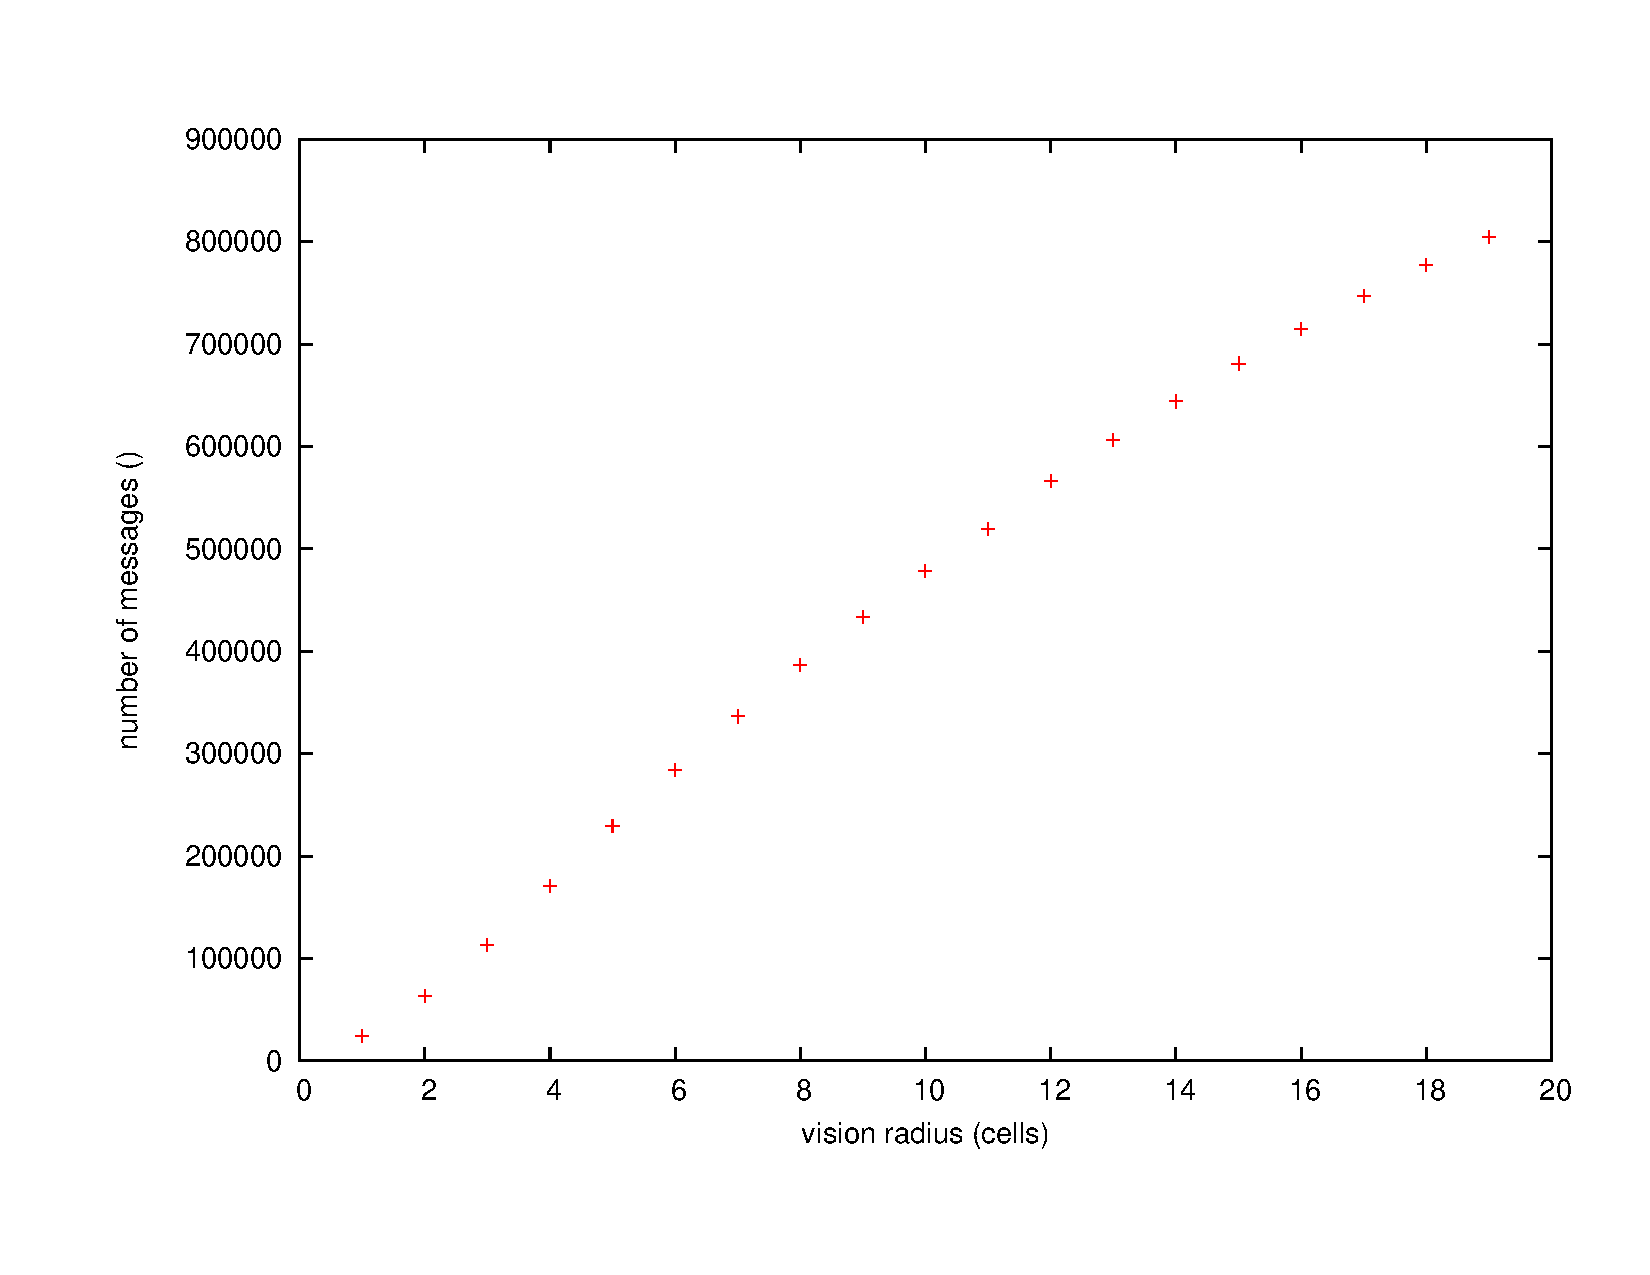
\includegraphics[scale=.3]{src/vision-message}
      \label{vision:message}
    }
    
    \subfigure[moyenne de place]{
      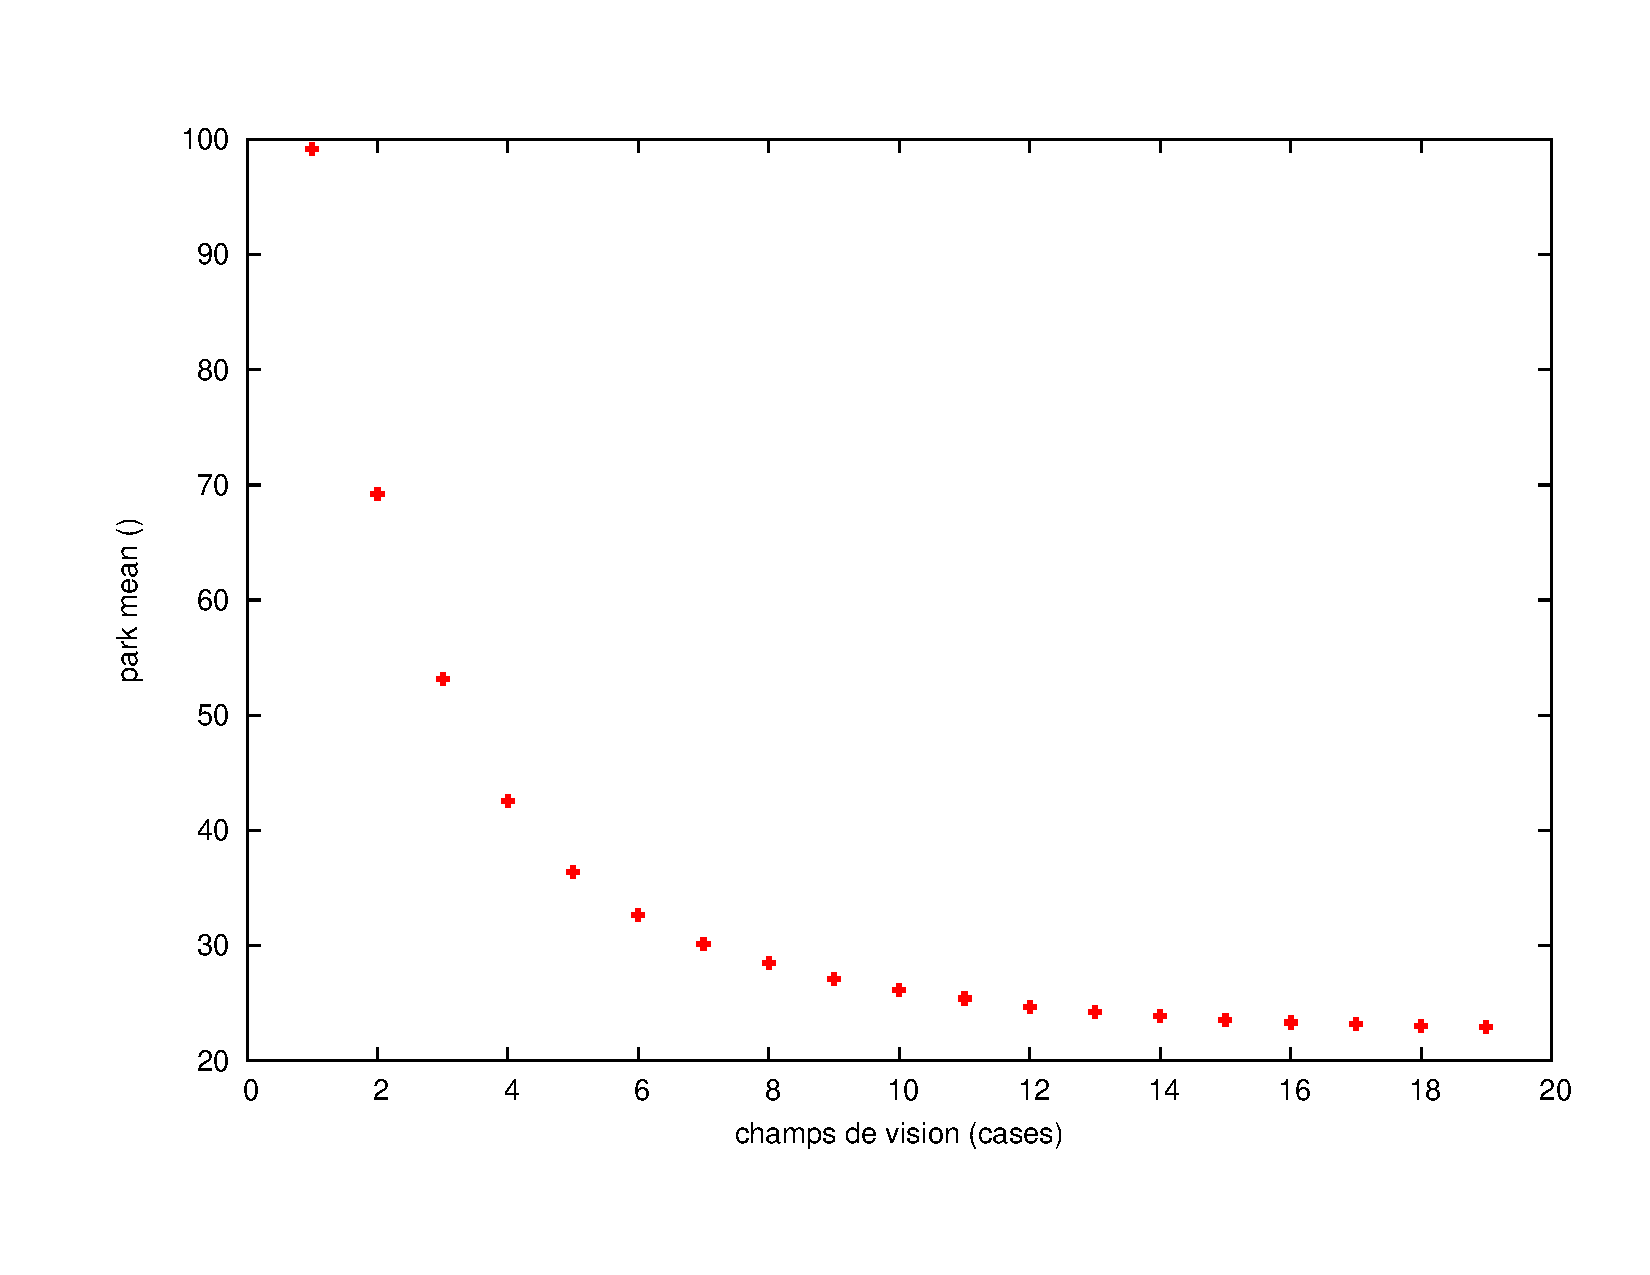
\includegraphics[scale=.3]{src/vision-seekfound}
      \label{vision:seekfound}
    }
    
    \subfigure[Ratio temps garé / temps total]{
      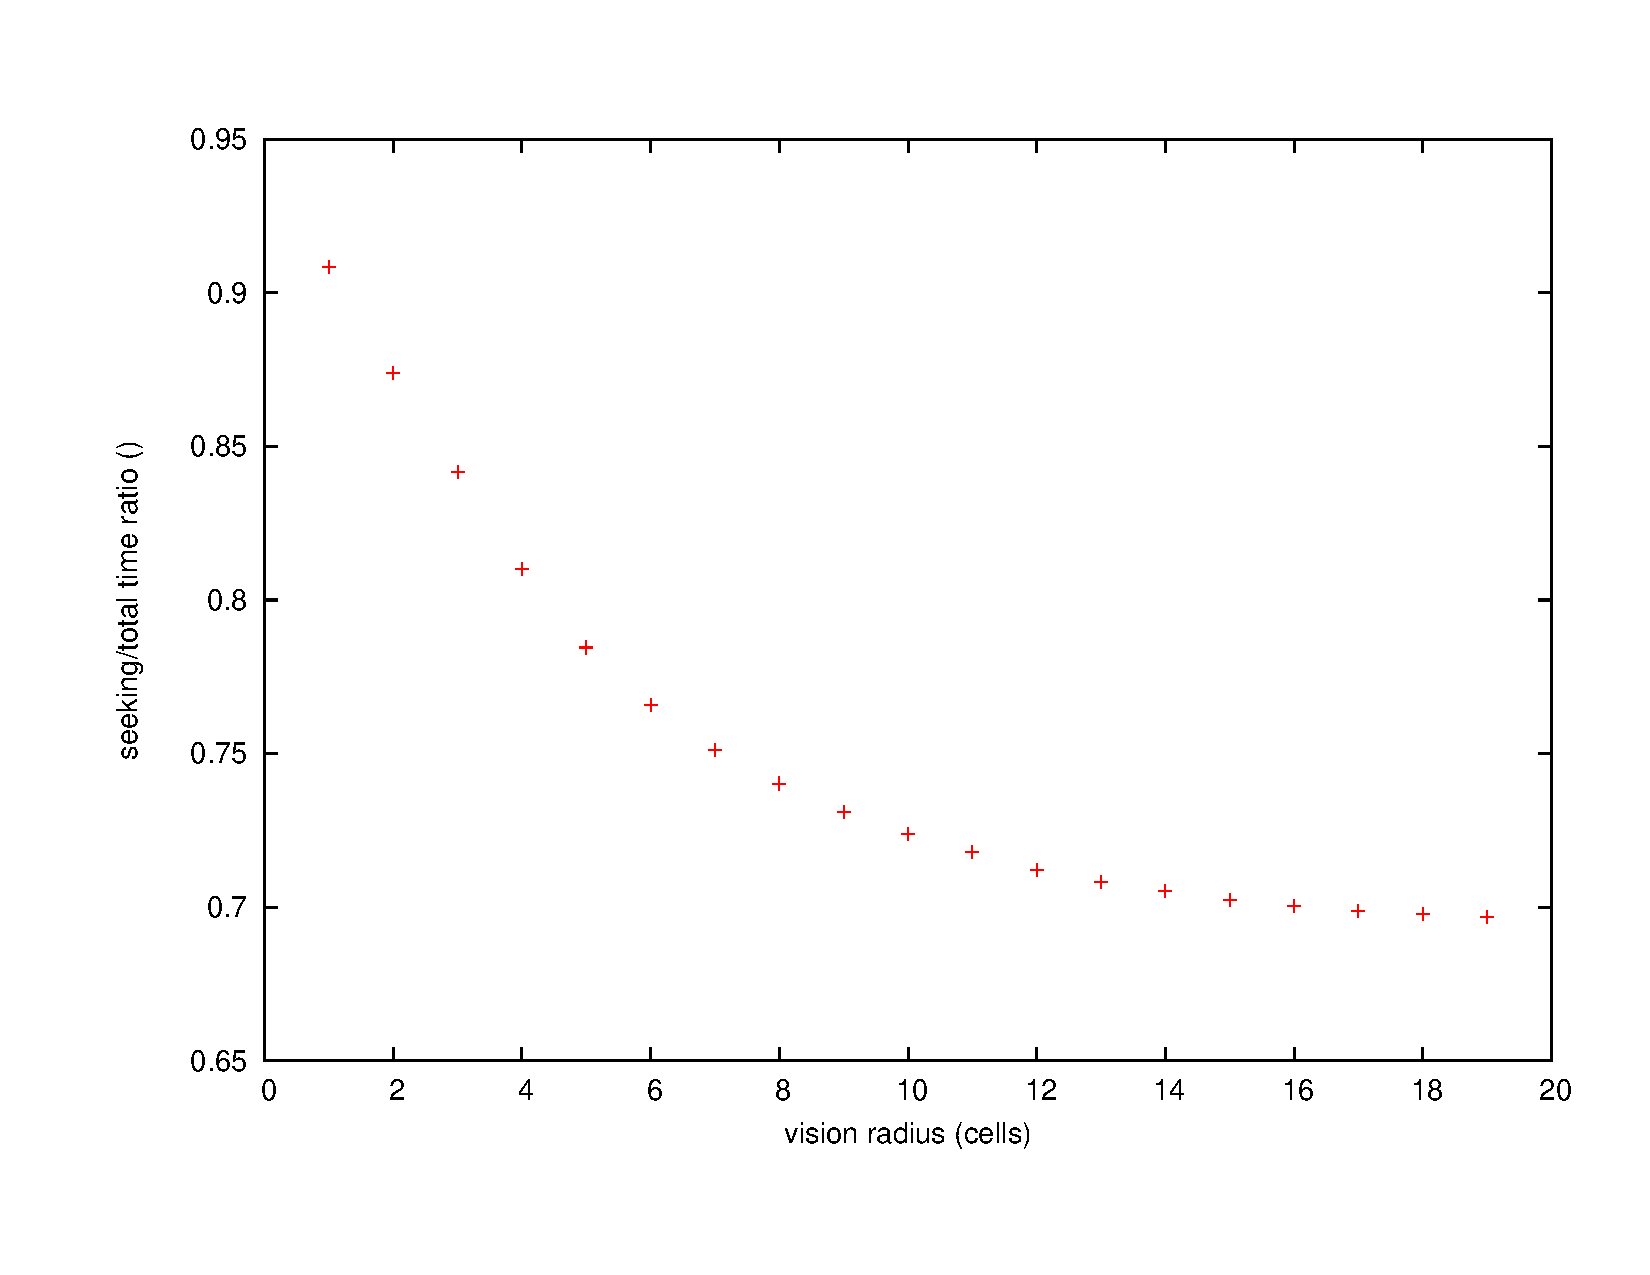
\includegraphics[scale=.3]{src/vision-seeking}
      \label{vision:seeking}
    }
  \end{center}

  \caption{Résultats obtenus en faisant varier le champs de visions}
  \label{vision:all}
\end{figure}

\subsubsection{Variation du temps de stationnement}

Deuxième paramètre à varier, le temps de stationnement, entre 0 et 15 rounds.

\paragraph{Résultats et interprétation}

Les résultats sont présentés dans la figure \ref{parktime:all}.
Le nombre de messages n'est pas vraiment influencé par le temps de stationnement.
En revanche on remarque que plus le temps de stationnement est long, plus la qualité de la solution trouvé par chaque agent se dégrade. Ceci s'explique par le fait que vu qu'il y a deux fois moins de places que de voitures, les places libres deviennent de plus en plus rares. Encore une fois avec d'autres paramètres par défaut cette courbe changerait. En l'état elle illustre bien un processus de famine et à l'inverse quand le temps de stationnement est faible, les solutions sont de meilleur qualité.\\

Enfin la solution générale s'améliore grandement (plus qu'avec le champs de vision) avec un temps de stationnement plus long. Ceci est la combinaison du temps de stationnement long améliorant le ratio et du phénomène de rarification des ressources l'améliorant encore plus.\\

Ce paramètres montre bien la dualité qu'il y a entre qualité globale de la solution du système et la qualité locale des solutions choisies par chaque agents.

\begin{figure}
  \begin{center}
    \subfigure[Nombre de messages en fonction du temps de stationnement]{
      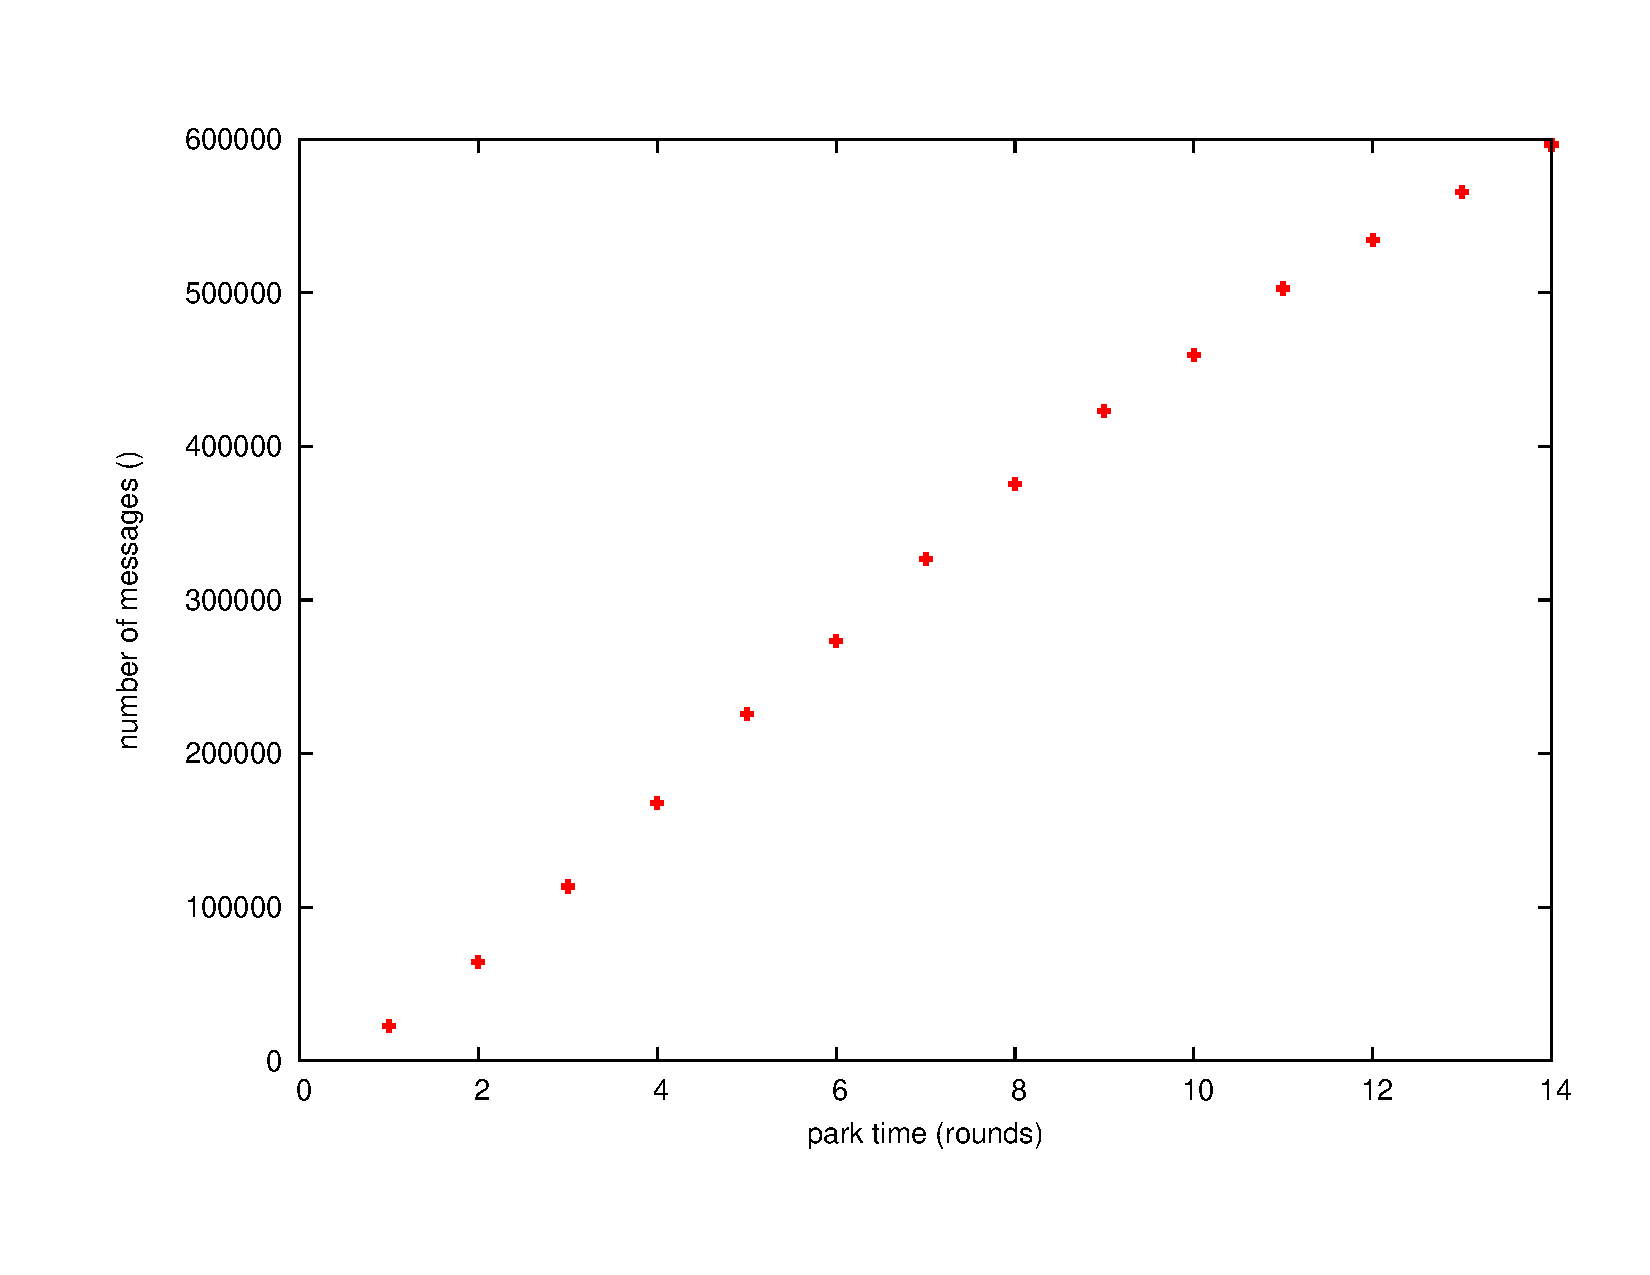
\includegraphics[scale=.3]{src/parktime-message}
      \label{parktime:message}
    }
    
    \subfigure[moyenne de place]{
      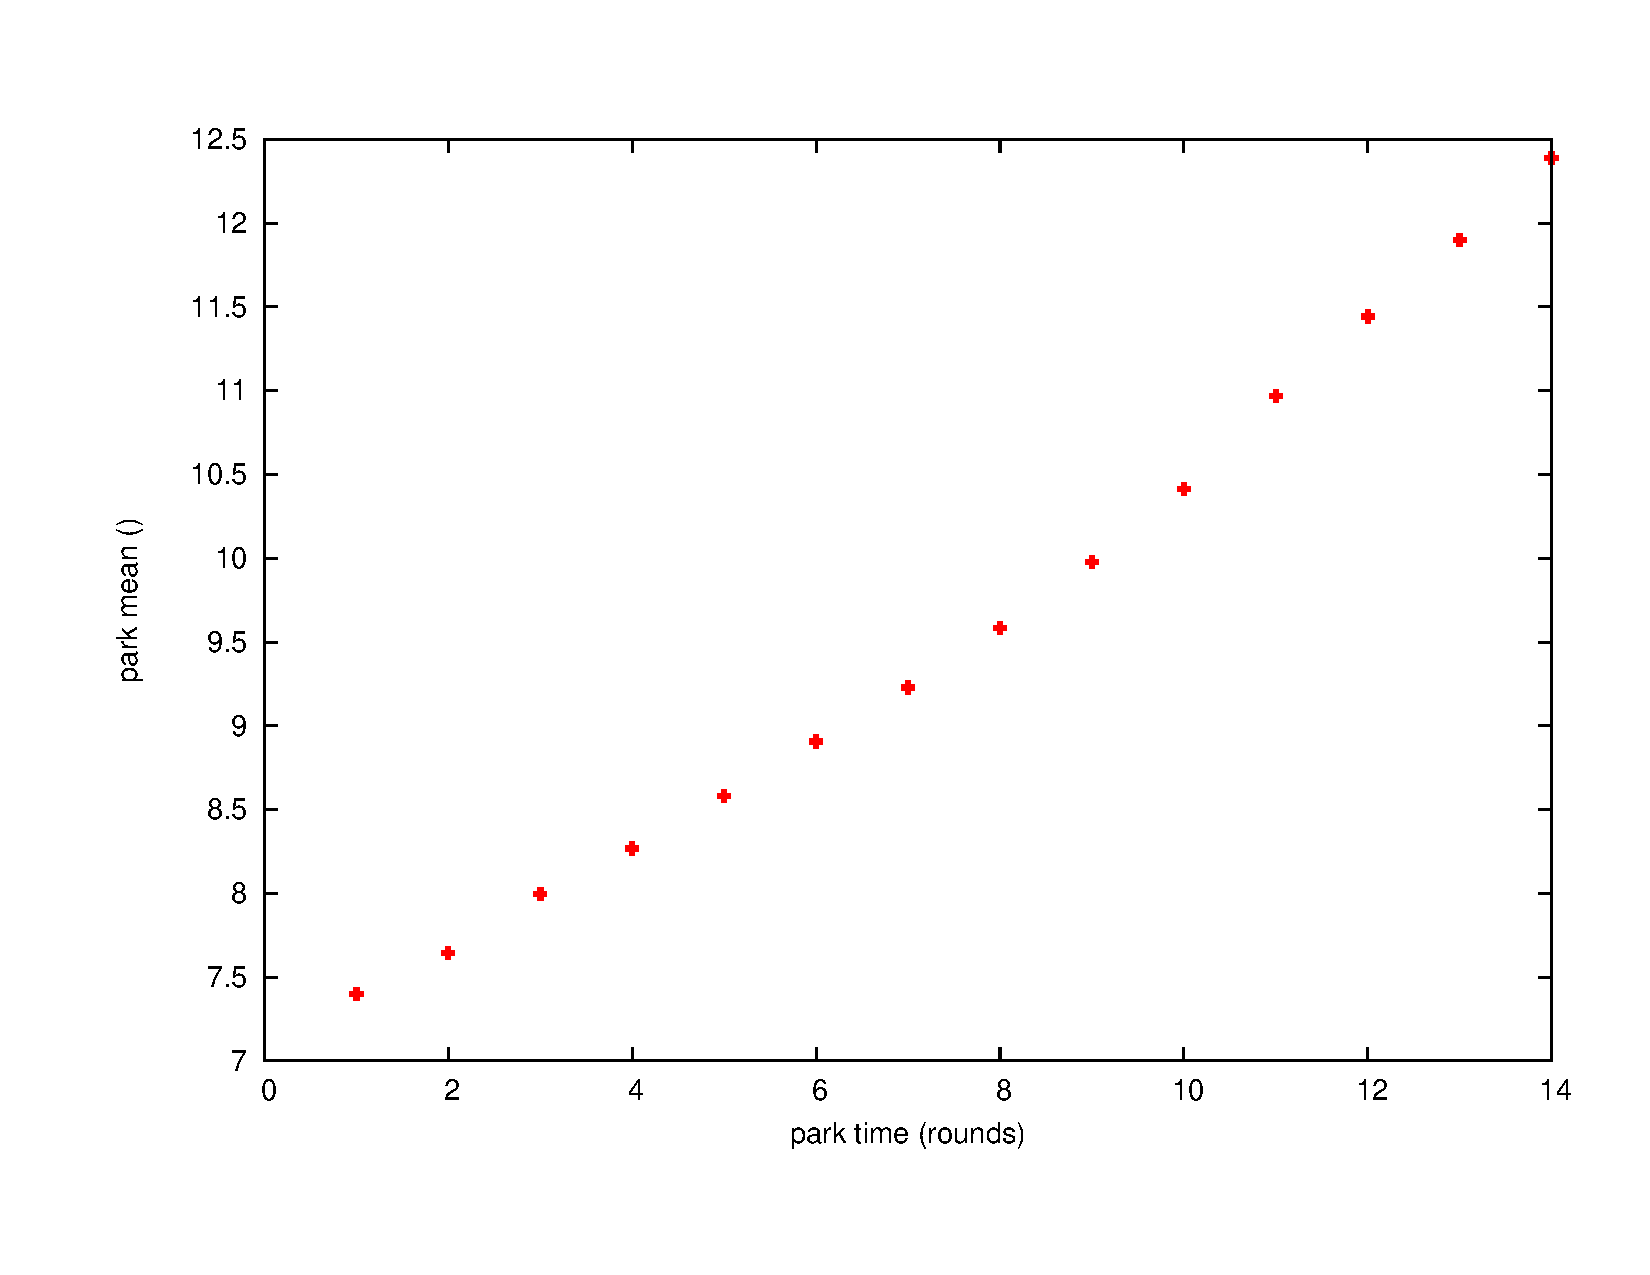
\includegraphics[scale=.3]{src/parktime-seekfound}
      \label{parktime:seekfound}
    }
    
    \subfigure[Ratio temps garé / temps total]{
      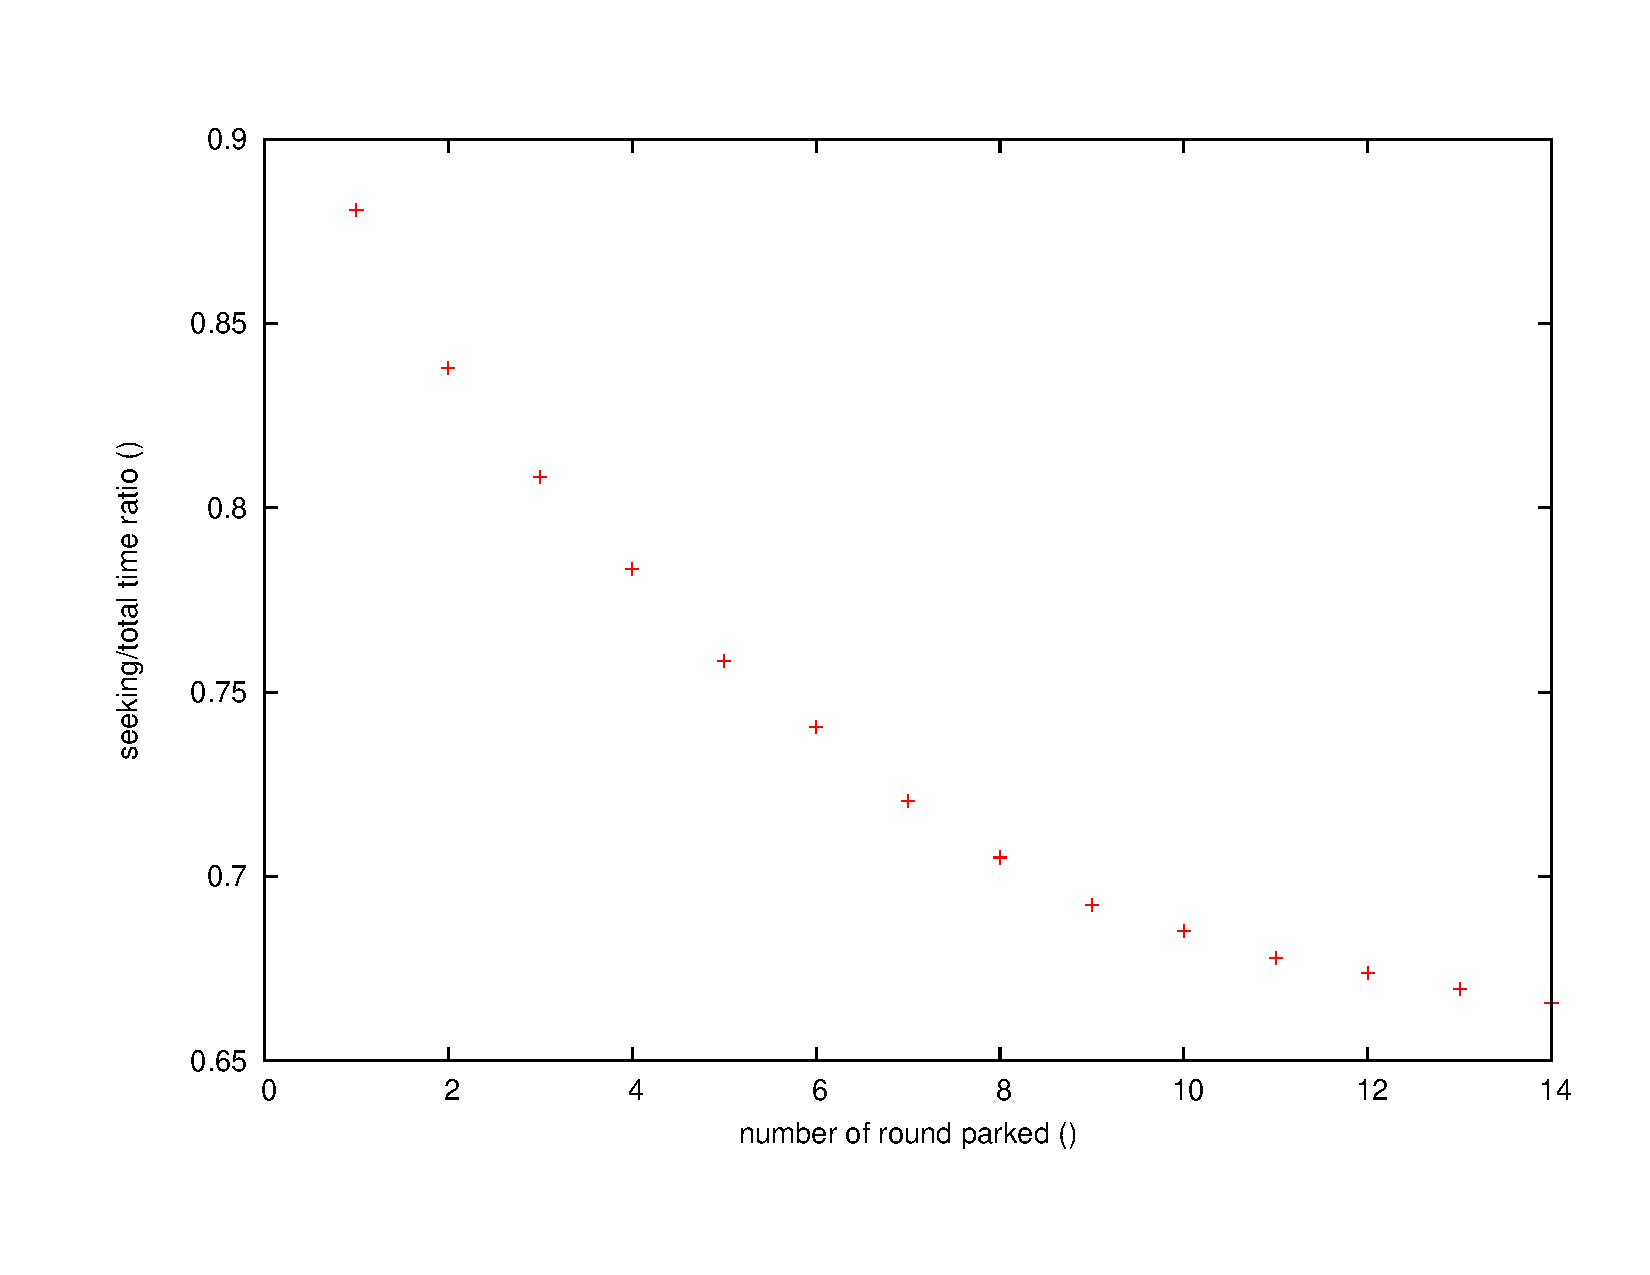
\includegraphics[scale=.3]{src/parktime-seeking}
      \label{parktime:seeking}
    }
  \end{center}

  \caption{Résultats obtenus en faisant varier le temps de stationnement}
  \label{parktime:all}
\end{figure}

\subsubsection{Temps de stationnement avant diffusion d'information}

Ce paramètre est spécifique à notre solution, c'est le nombre de rounds avant la fin du stationnement a partir duquel on va commencer à signaler que la place va se libérer. Ce temps est donné en nombre de rounds avant la fin du stationnement, entre 1 et 10.


\paragraph{Résultats et interprétation}

Les résultats sont présentés dans la figure \ref{timeb4broad:all}\\

{\bf Note: } Plus le temps avant diffusion est faible, plus l'agent va prévenir tard avant de quitter sa place. Ainsi avec un temps de 1 round l'agent prévient les autres 1 round avant de quitter sa place.\\

L'augmentation du nombre de messages envoyés s'explique simplement par le fait qu'à chaque round encore sur une place si il a commencé à diffuser l'agent continue à le faire. Plus il diffuse tard moins il le fait longtemps d'où moins de messages envoyés. C'est le paramètre influençant le plus le nombre de messages transmis.\\

Par contre, plus les autres agents sont prévenus tard, moins il ont le temps de réagir donc plus la qualité locale et totale des solutions décroît. A noter quand même que la solution globale s'améliore plus que la solution locale quand le paramètre varie. Cela peut être du au phénomène de rarification des ressources propre à notre système.

\begin{figure}
  \begin{center}
    \subfigure[Nombre de messages en fonction du temps avant diffusion]{
      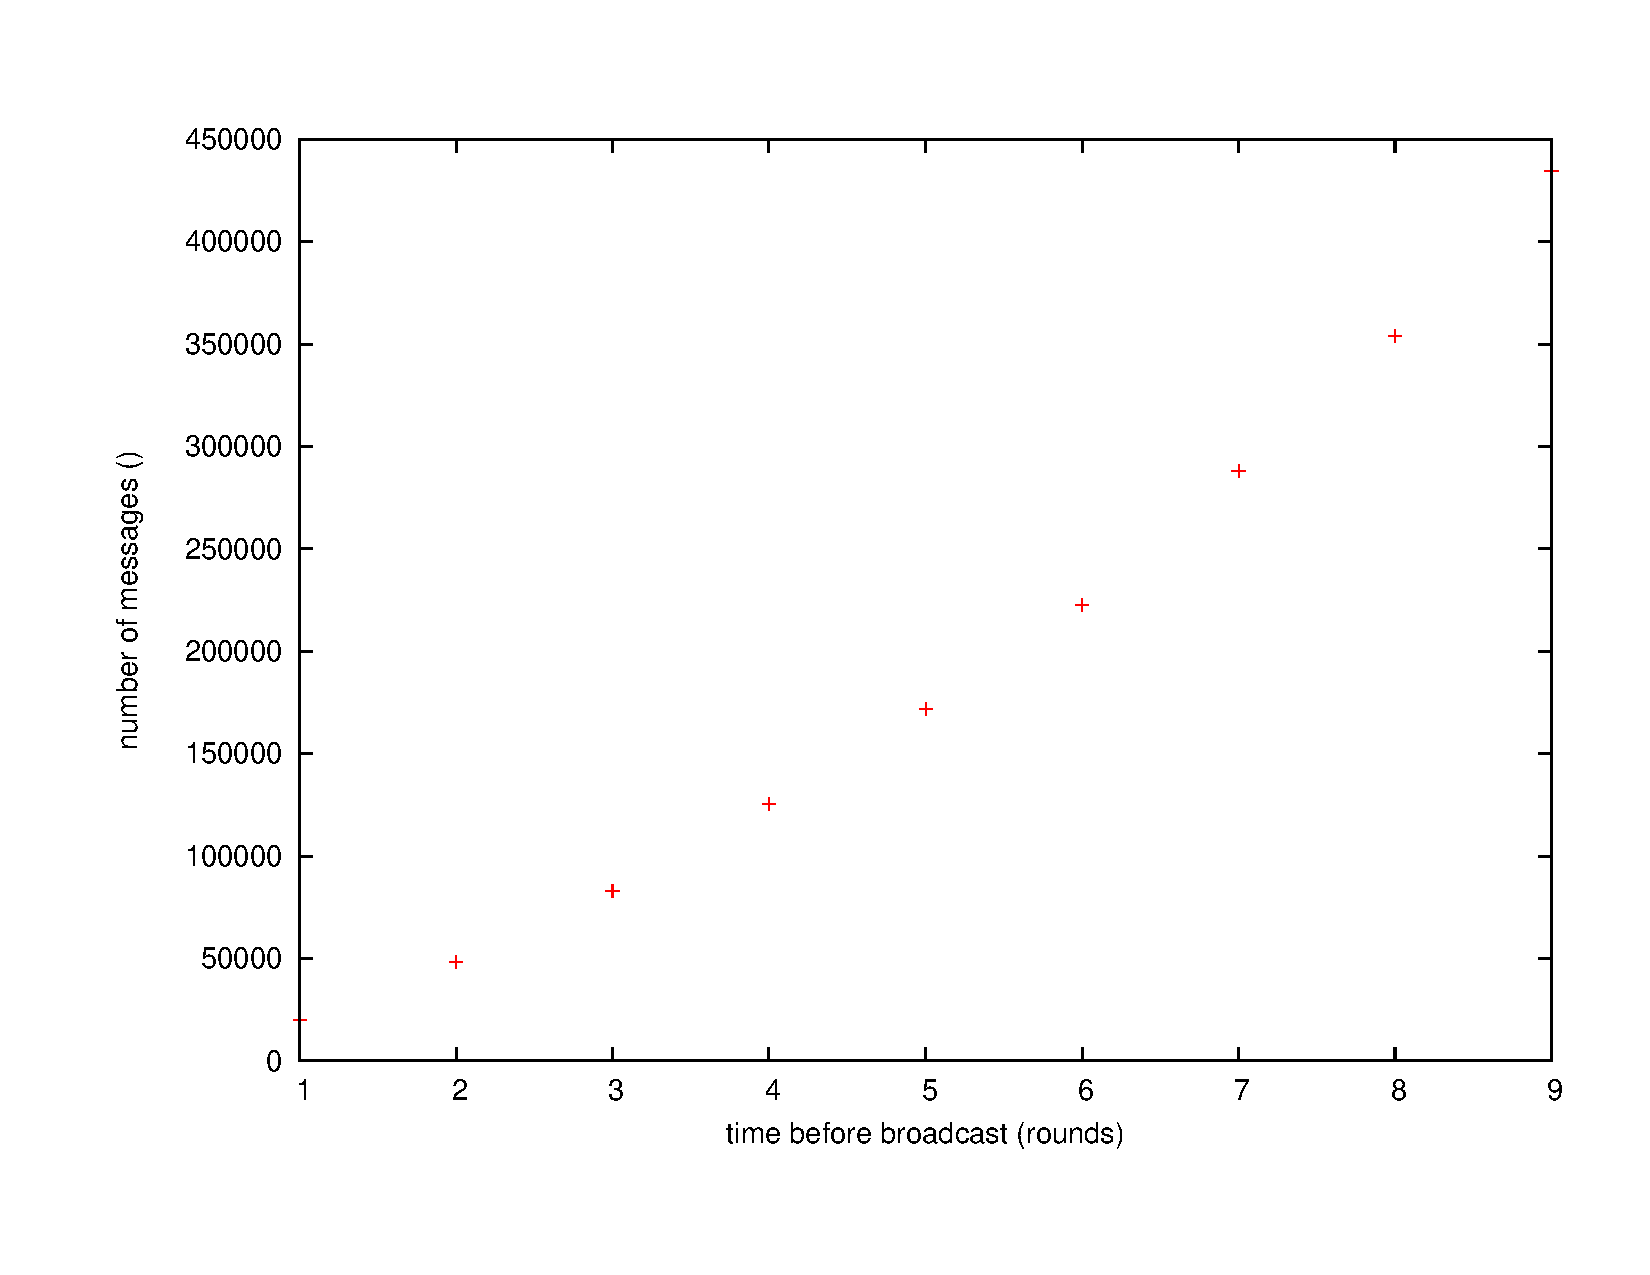
\includegraphics[scale=.3]{src/timeb4broad-message}
      \label{timeb4broad:message}
    }
    
    \subfigure[Moyenne de place]{
      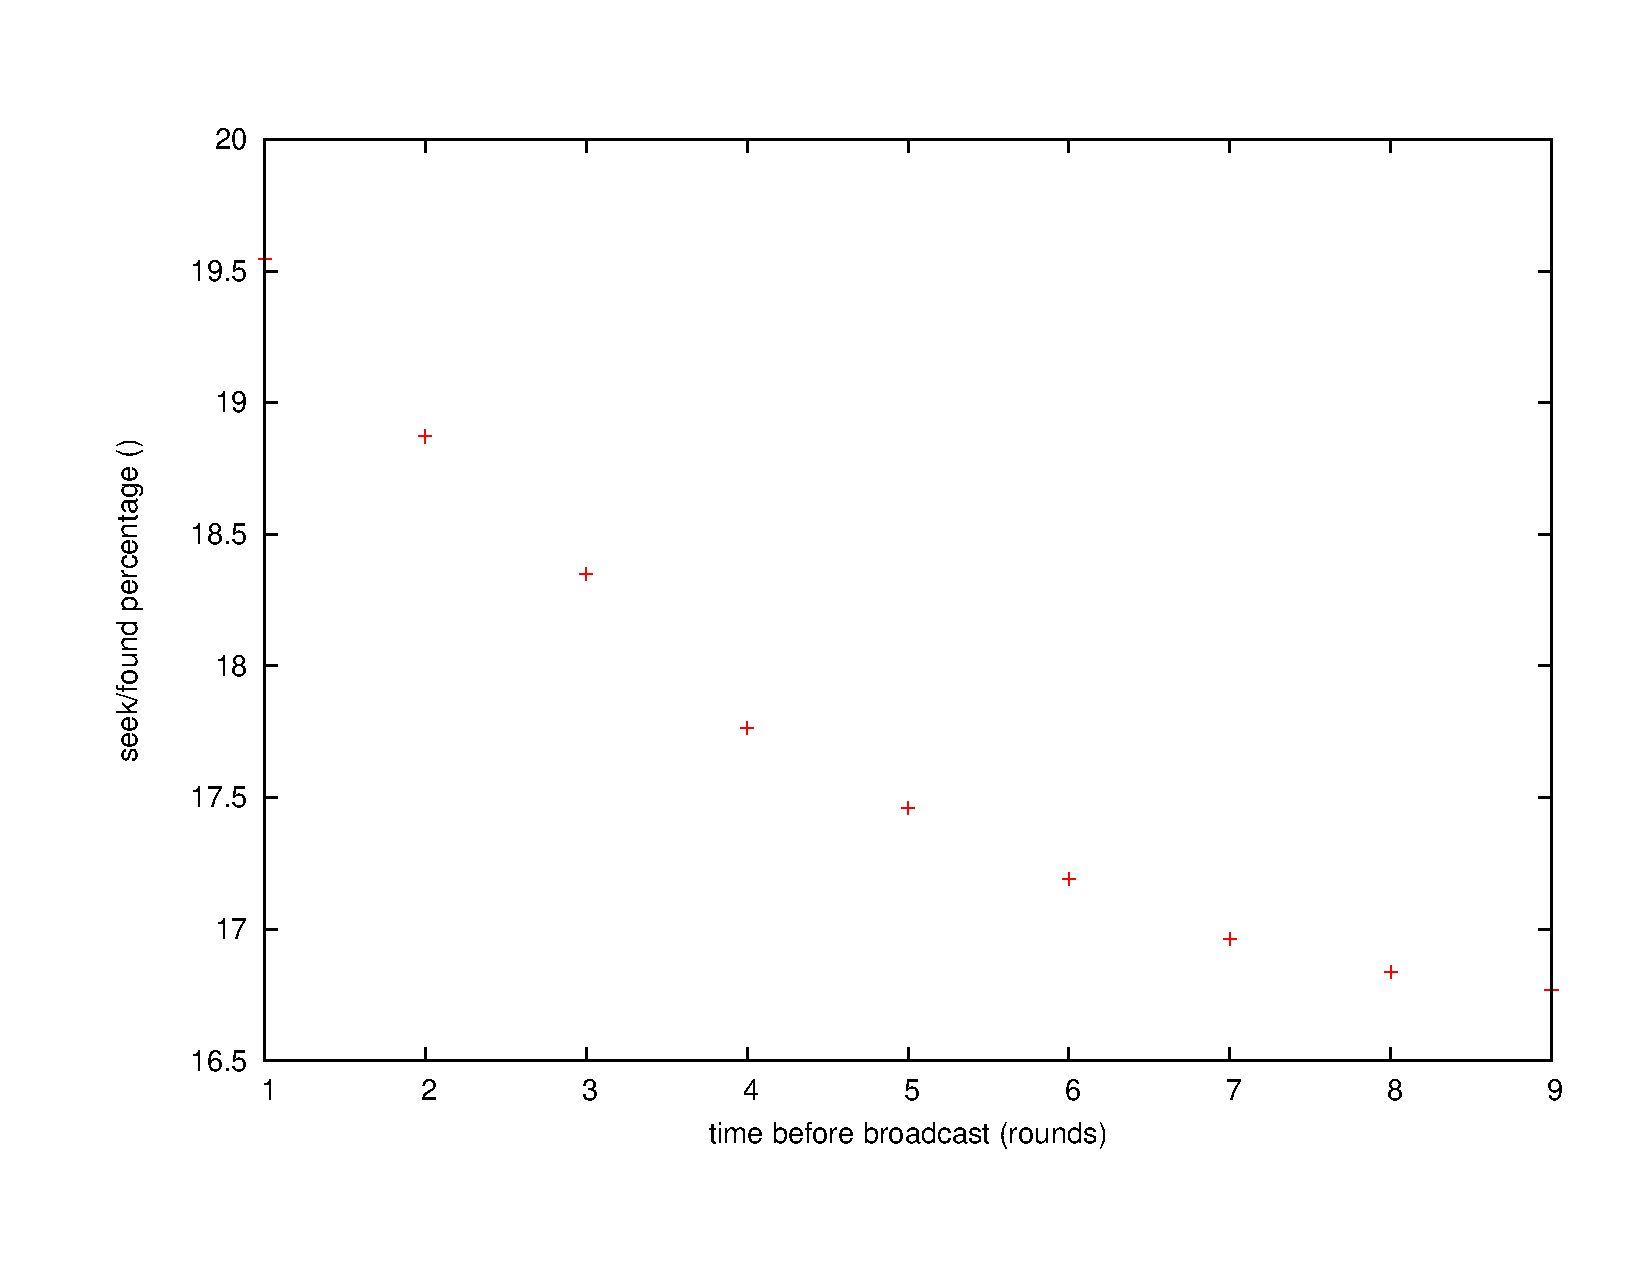
\includegraphics[scale=.3]{src/timeb4broad-seekfound}
      \label{timeb4broad:seekfound}
    }
    
    \subfigure[Ratio temps garé / temps total]{
      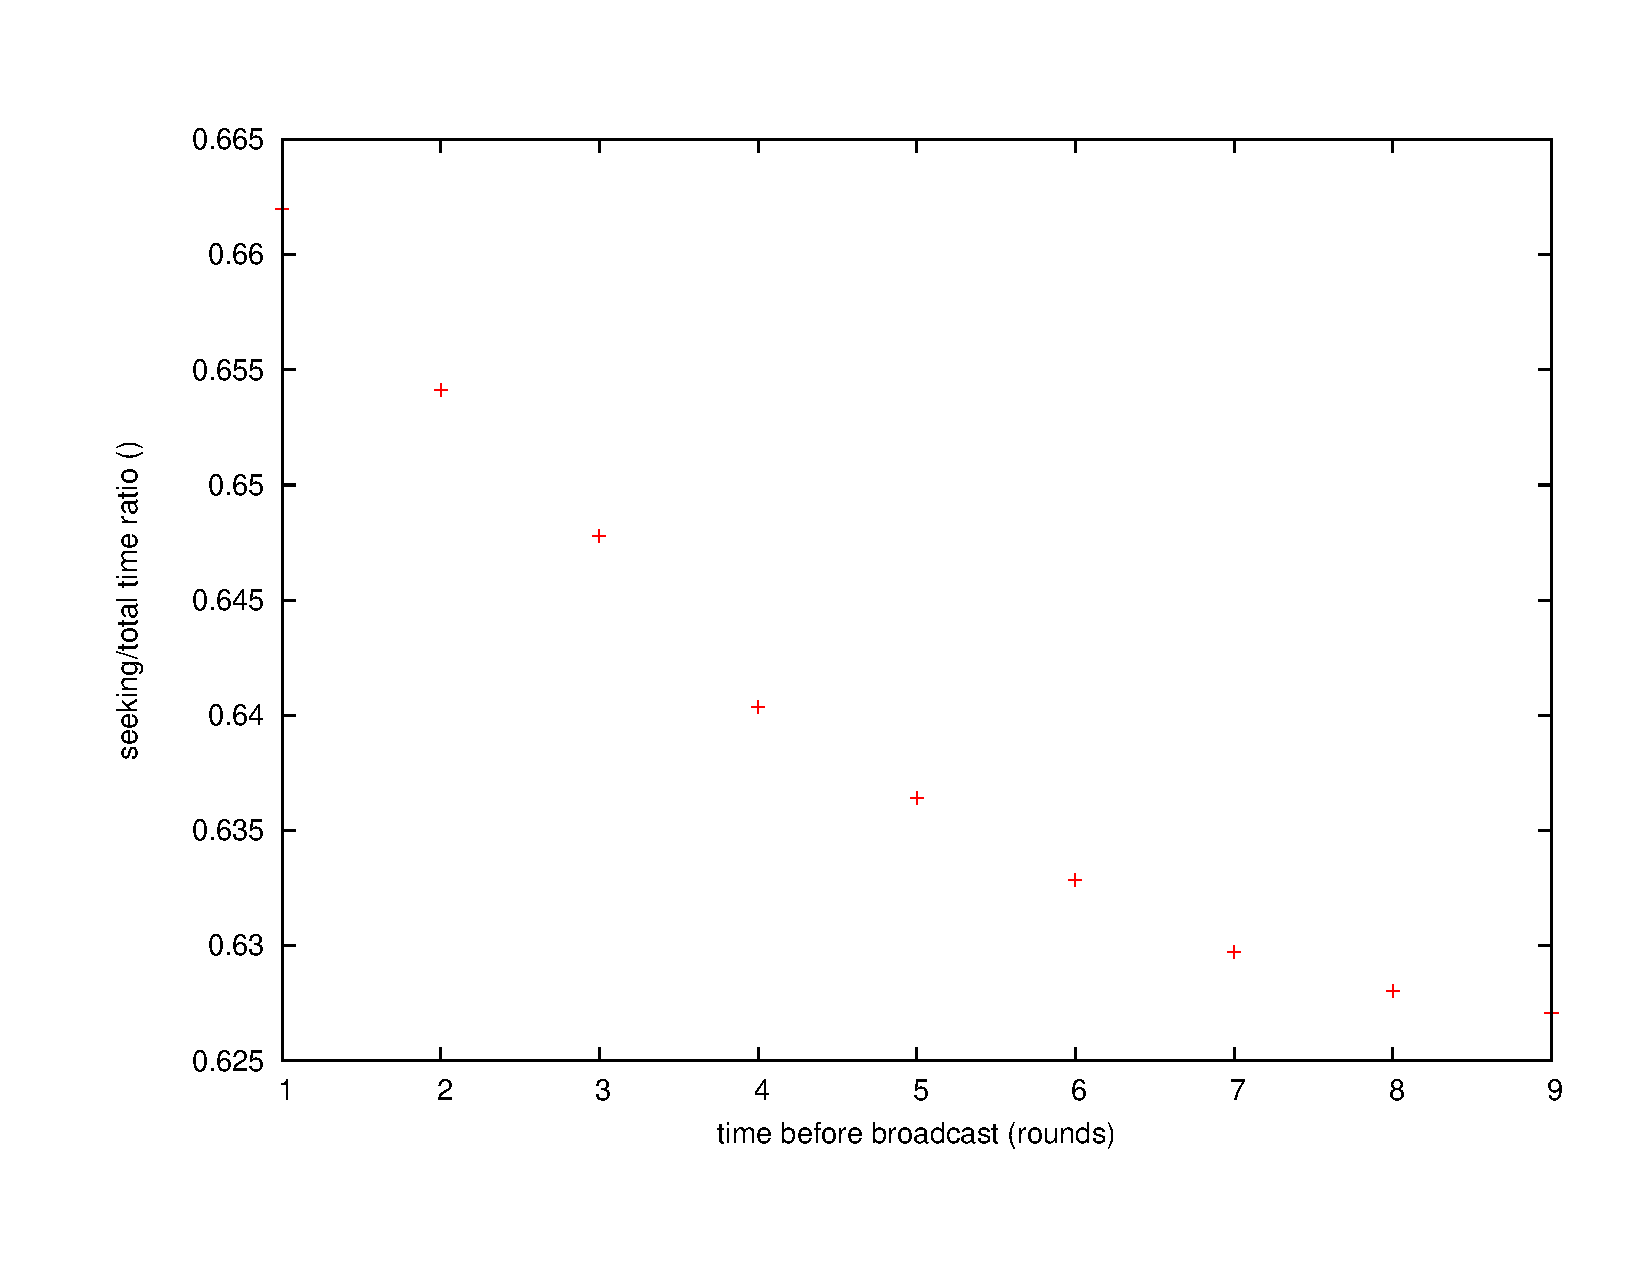
\includegraphics[scale=.3]{src/timeb4broad-seeking}
      \label{timeb4broad:seeking}
    }
  \end{center}

  \caption{Résultats obtenus en faisant varier le temps avant diffusion}
  \label{timeb4broad:all}
\end{figure}

\subsubsection{Variation du temps avant recherche}

Finalement, le dernier paramètre local à notre système est le temps qu'un agent met avant de se remettre à la recherche d'une place après en avoir quitté une. C'est ce qu'on peut appeler un paramètre d'équité, il est censé assurer qu'aucun agent ne monopolise de ressources.

\paragraph{Résultats et interprétation}

Les résultats sont présentés dans la figure \ref{timeb4search:all}\\

C'est le paramètre qui donne les résultats les plus intéressants. Tout d'abord le nombre de messages augmente linéairement par rapport au temps avant une nouvelle recherche. En effet, plus les agents s'éloignent de leur position de stationnement, plus ils vont explorer le terrain et donc trouver d'autres places.\\

Les deux courbes de ratios montrent une forme non rencontrée jusqu'à présent. Les solutions locales et globales commencent par se détériorer pour s'améliorer de manière remarquable. Cela s'explique en comprenant que les faibles valeurs provoquent un phénomène d'appropriation des places qui reviennent toujours au même agent. Les fortes valeurs elles correspondent à une équité forte, les agents s'éloignent suffisamment de leur ancienne place pour ne plus retourner dessus tout de suite après laissant la place à un autre agent. La perte de performance est du à un éloignement fort provoquant une perte de temps pour retourner sur la place mais trop faible pour qu'un autre agent ou une autre place soit trouvé.\\

Finalement, plus les agents se dispersent sur la grille meilleur sont les solutions locales et globales. Ceci se payant malheureusement par un fort nombre de messages échangés.

\begin{figure}
  \begin{center}
    \subfigure[Nombre de messages en fonction du temps avant une nouvelle recherche]{
      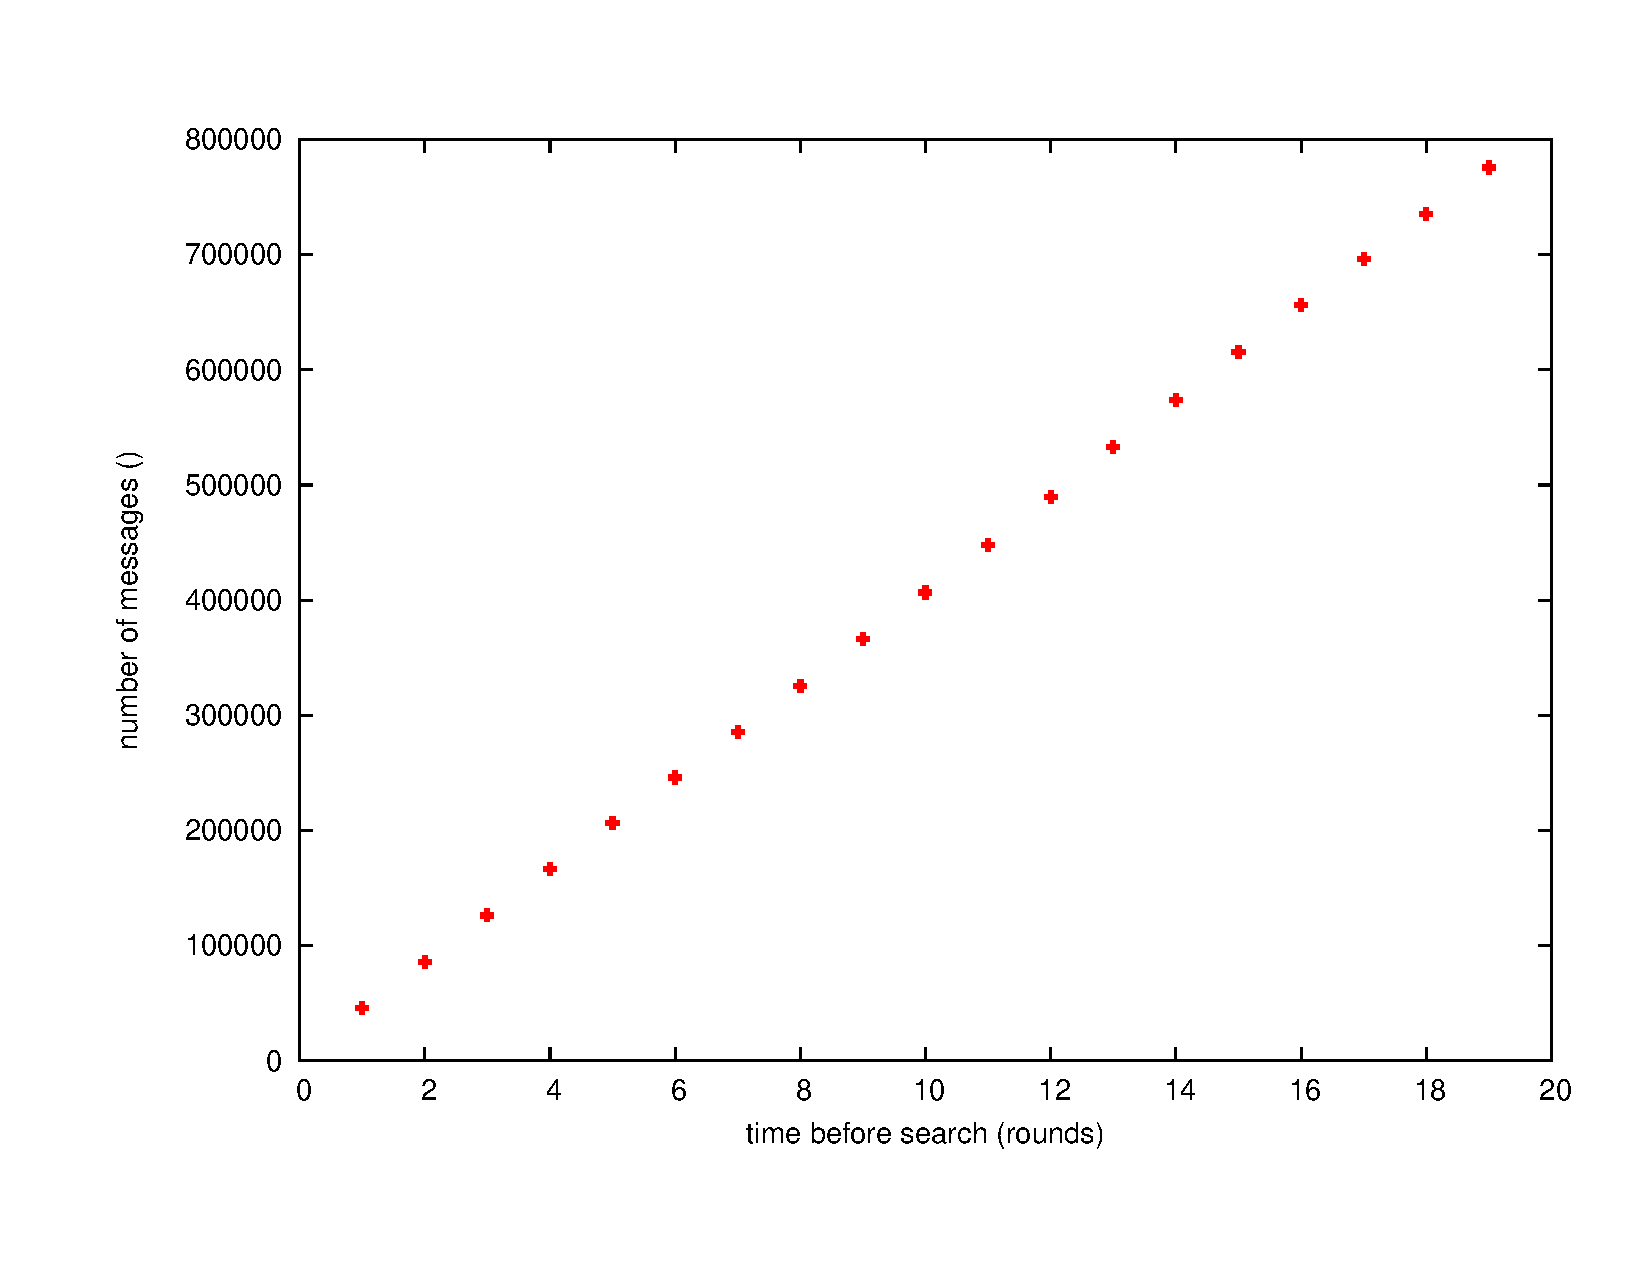
\includegraphics[scale=.3]{src/timeb4search-message}
      \label{timeb4search:message}
    }
    
    \subfigure[Moyenne de place]{
      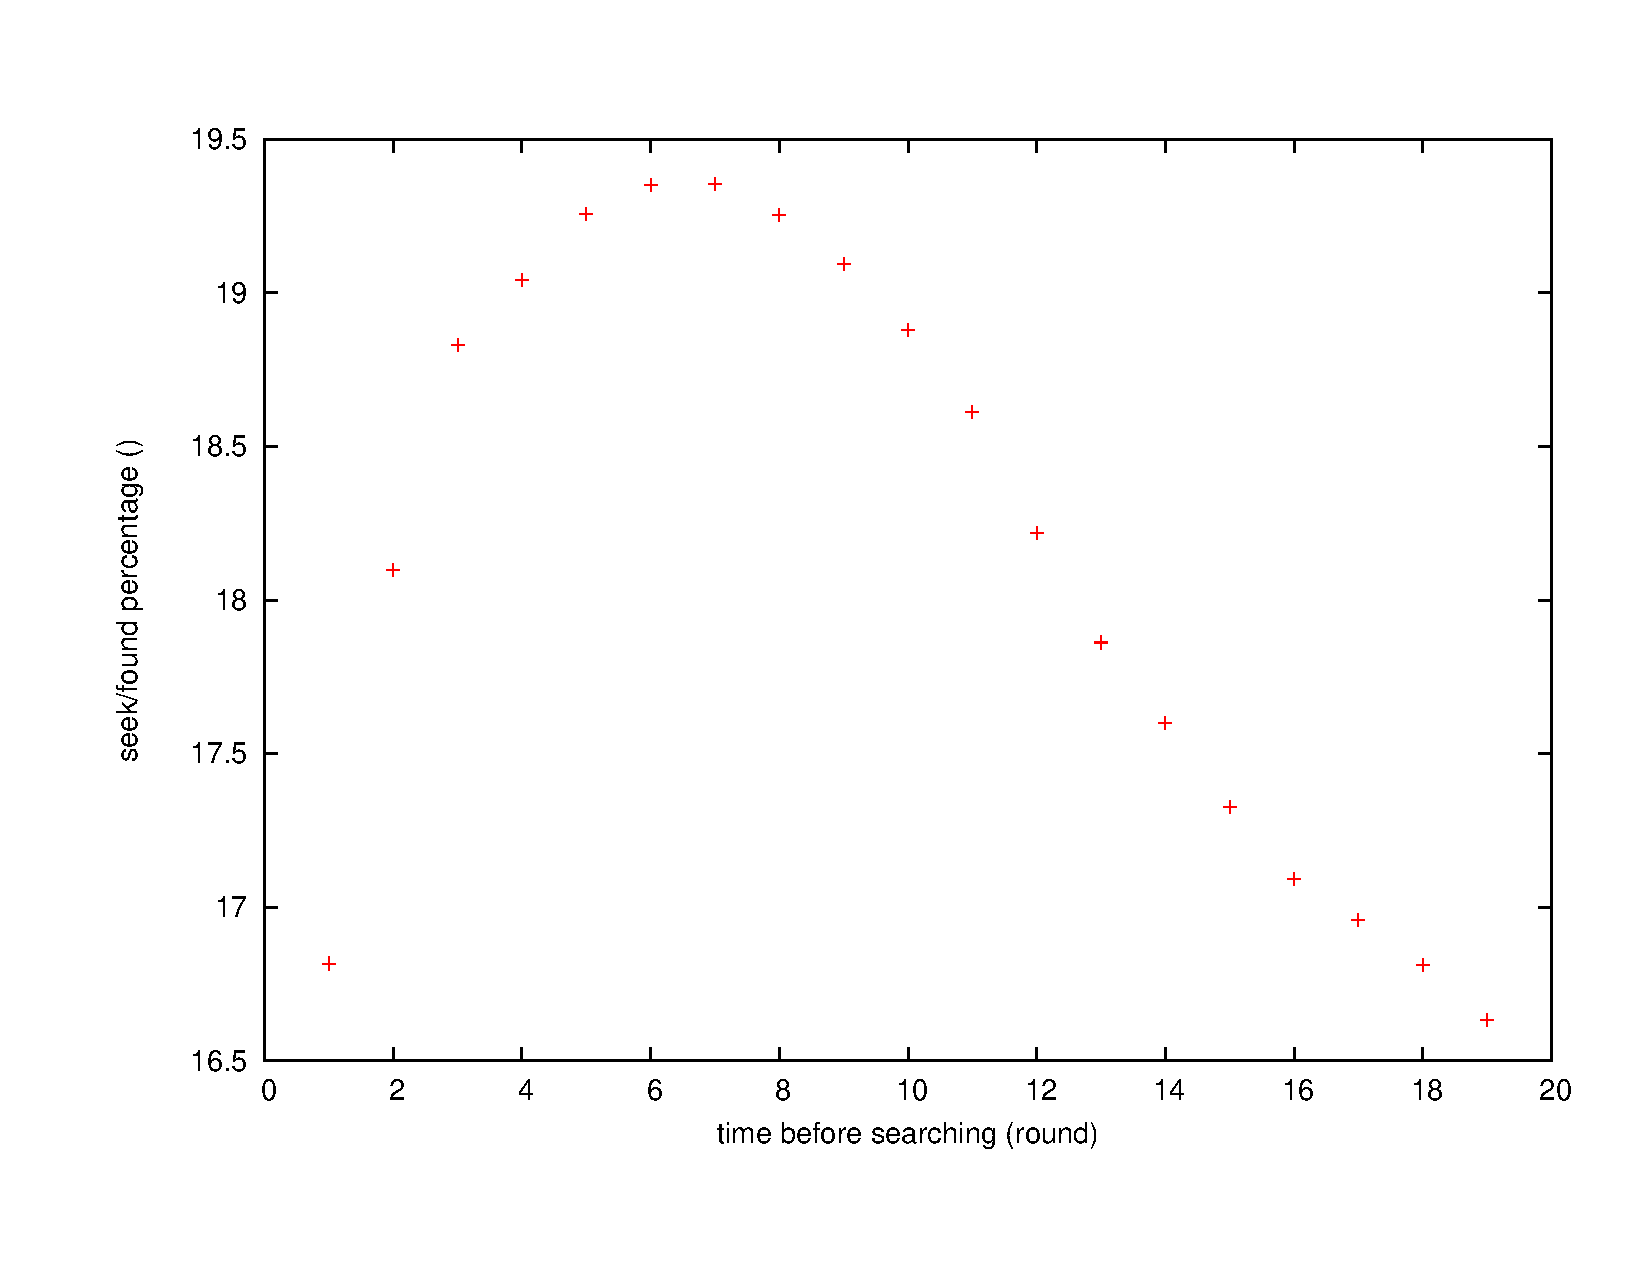
\includegraphics[scale=.3]{src/timeb4search-seekfound}
      \label{timeb4search:seekfound}
    }
    
    \subfigure[Ratio temps garé / temps total]{
      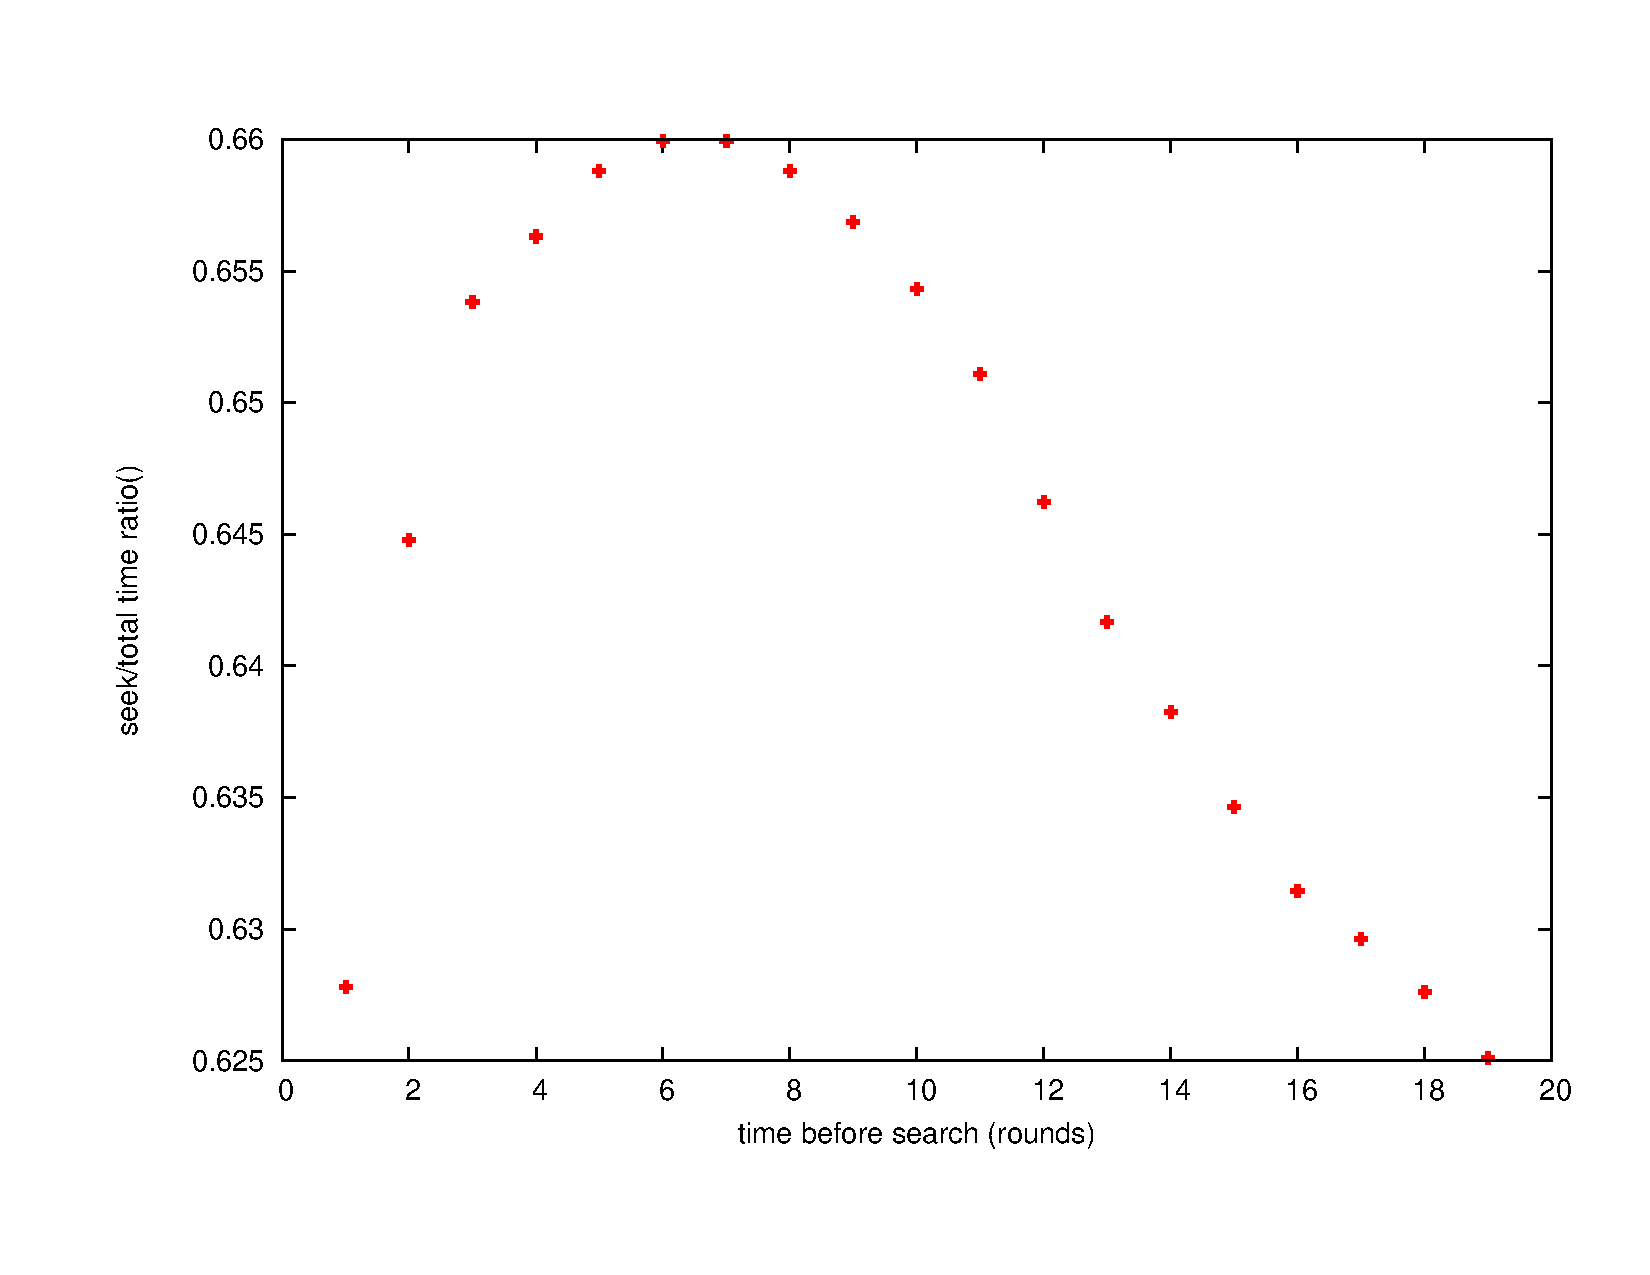
\includegraphics[scale=.3]{src/timeb4search-seeking}
      \label{timeb4search:seeking}
    }
  \end{center}

  \caption{Résultats obtenus en faisant varier le temps avant une nouvelle recherche}
  \label{timeb4search:all}
\end{figure}

\subsection{Paramètres du système}

Cette fois nous faisons varier le nombre d'agents et le nombre de places disponibles. La seule contrainte étant qu'il y aille toujours moins de places que de voitures.

\subsubsection{Nombre de voitures et nombre de places}

Deux paramètres évalués ici sont le dimensionnement du système et le ratio voitures / places.
Les résultats sont présentés dans la figure \ref{nbagents:all}.\\

Il est intéressant de voir que le ratio voitures / places n'influence que très faiblement notre système.
Ceci est du à un phénomène de stabilisation du système dans lequel chaque agent trouve une place en un temps borné.\\

Un phénomène très intéressant est l'amélioration de la solution avec le nombre d'agents. Cela prouve une bonne communication et prise en compte des informations entre agents. De plus changer le nombre de places pour un nombre d'agents donné n'a que très peu d'impact sur le système ce qui prouve une forme de robustesse.

\begin{figure}
  \begin{center}
    \subfigure[Nombre de messages en fonction des nombres d'agents et de places]{
      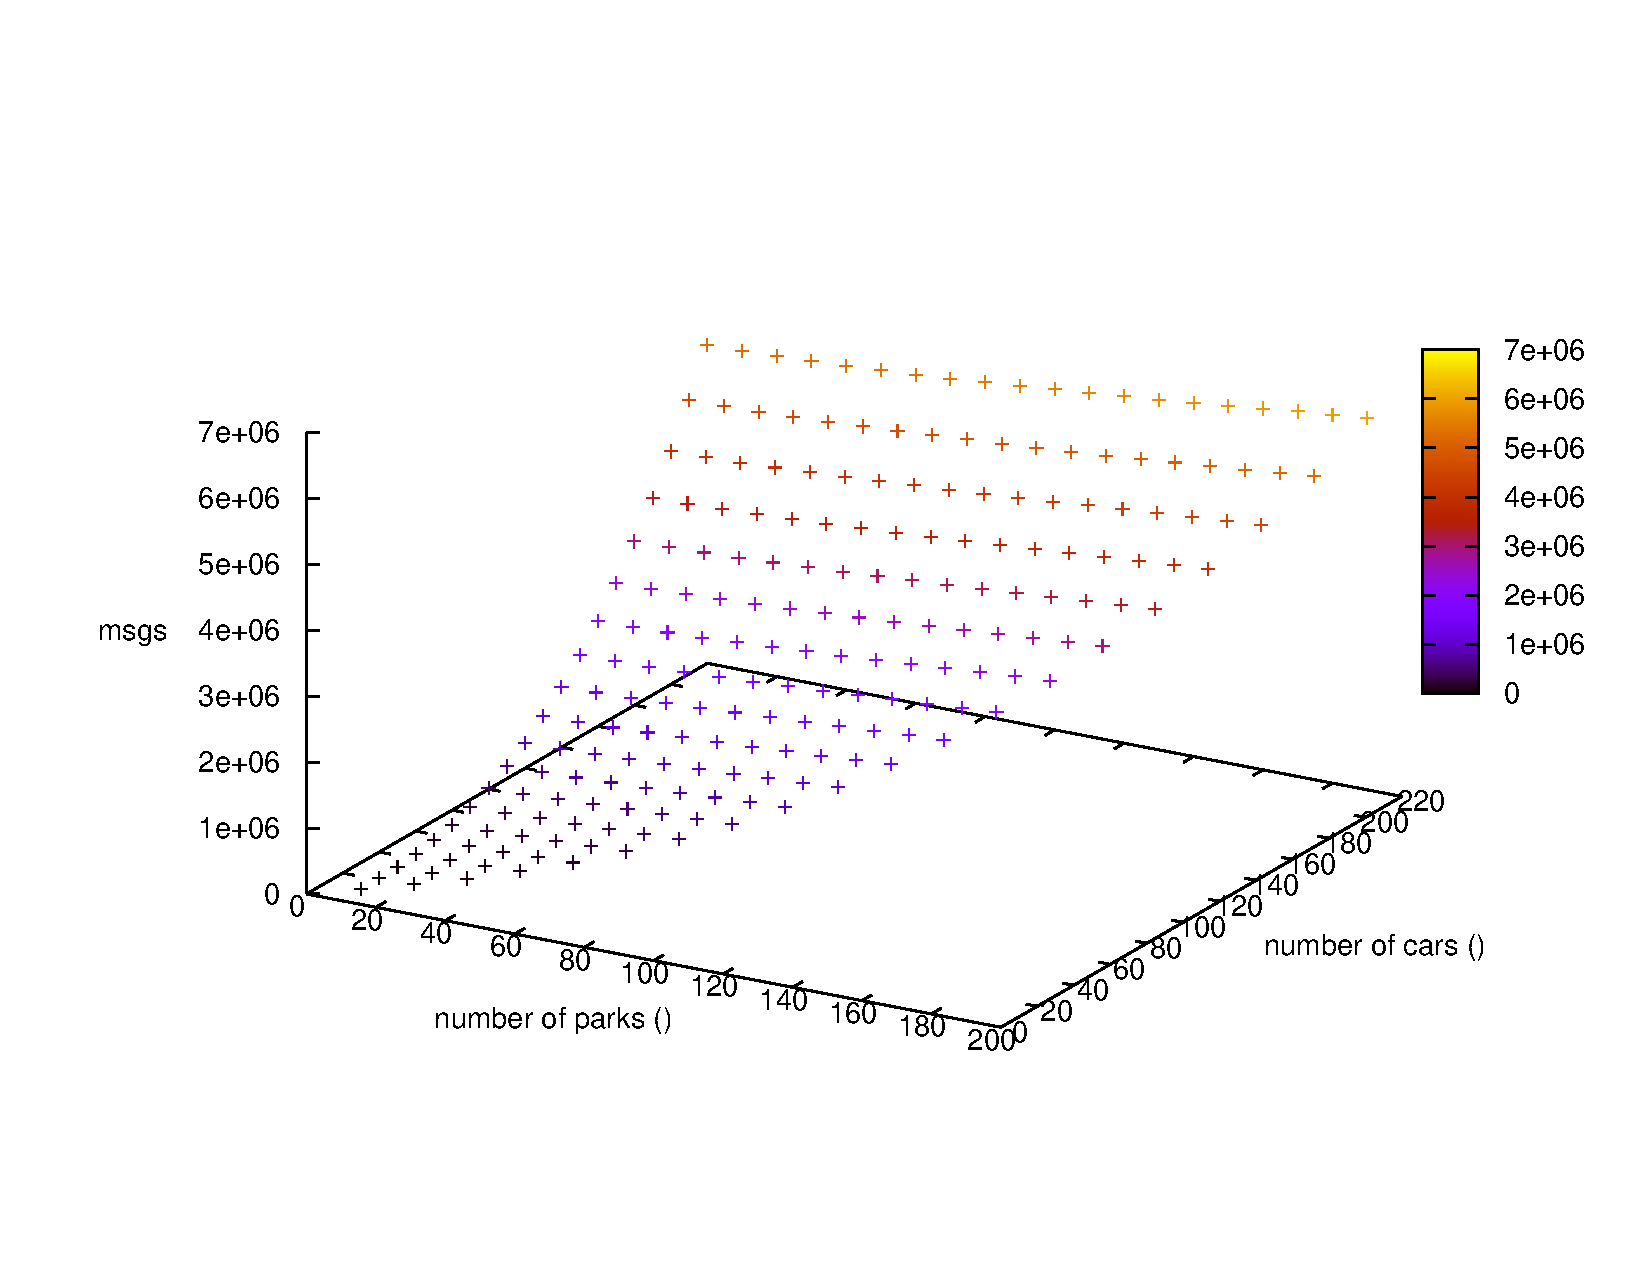
\includegraphics[scale=.35]{src/nbagents-message}
      \label{nbagents:message}
    }
    
    \subfigure[Moyenne de place]{
      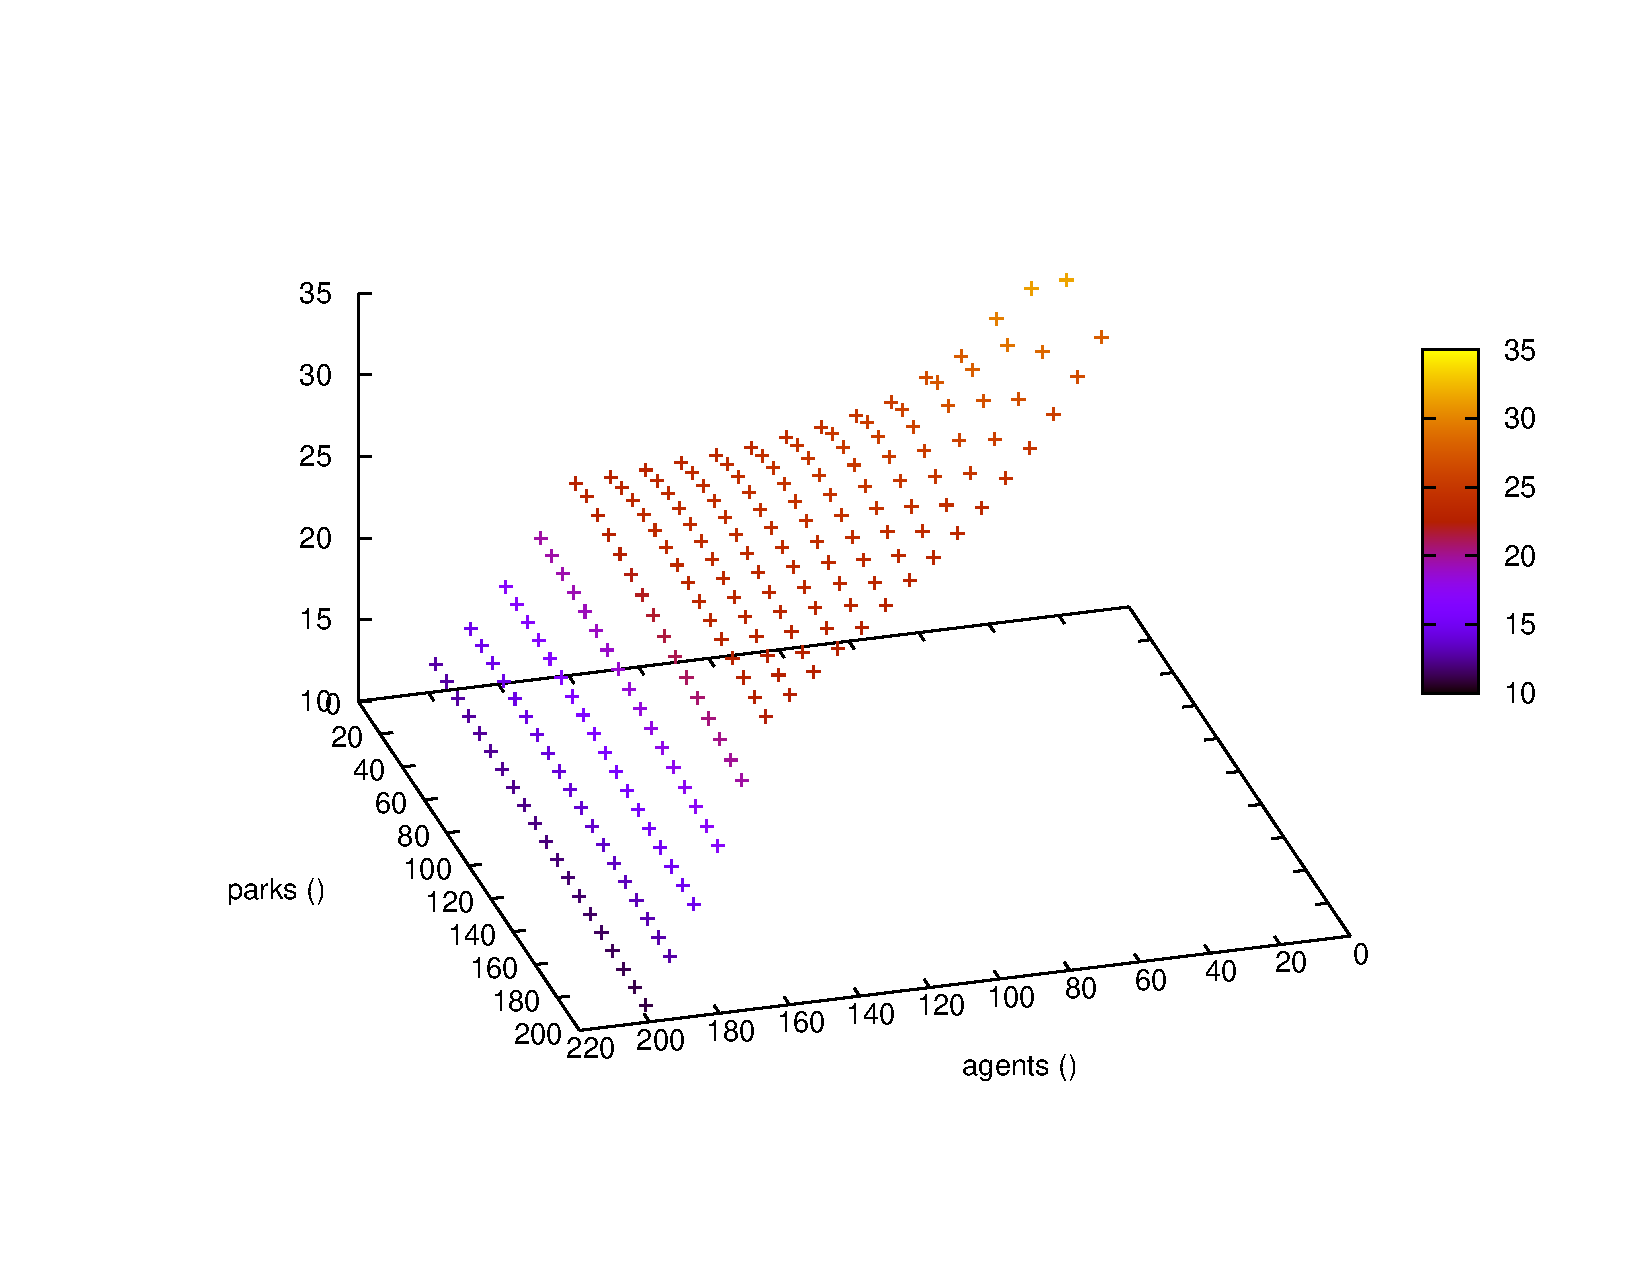
\includegraphics[scale=.35]{src/nbagents-seekfound}
      \label{nbagents:seekfound}
    }
    
    \subfigure[Ratio temps garé / temps total]{
      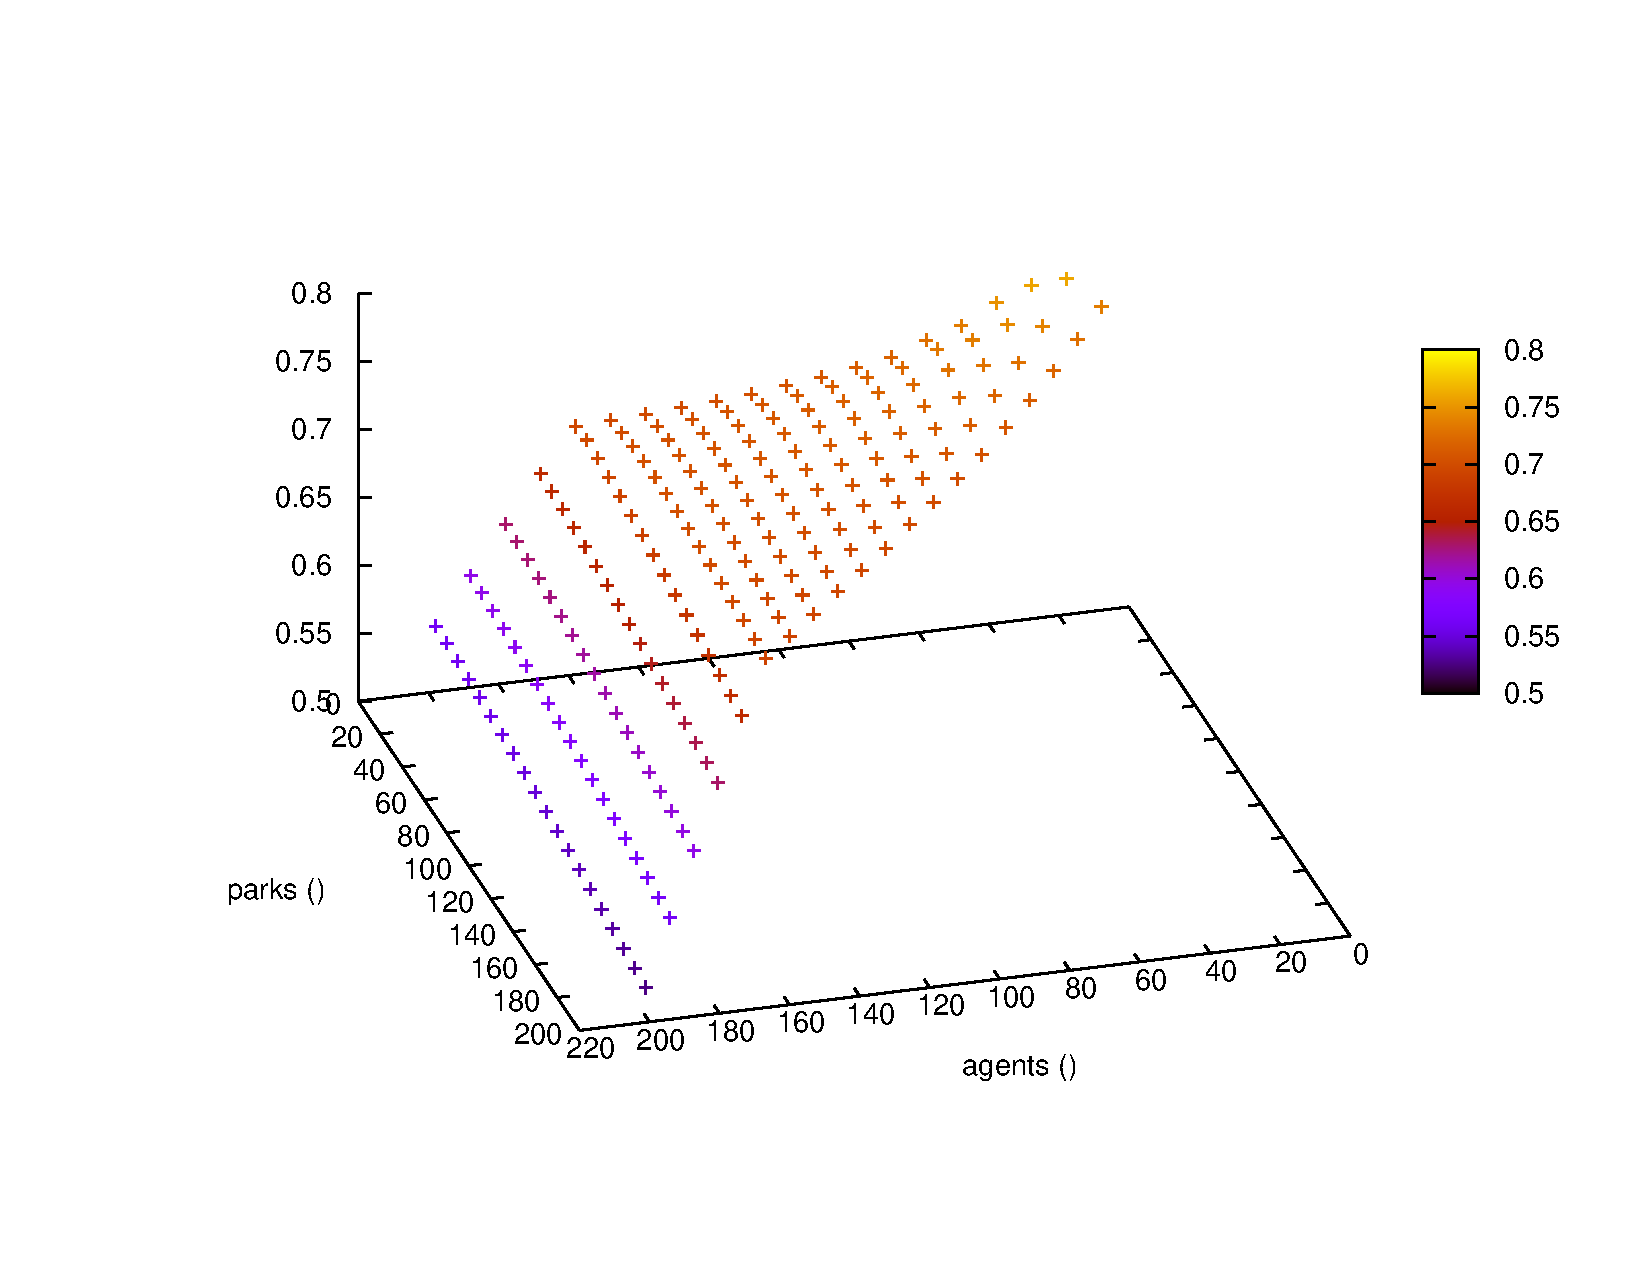
\includegraphics[scale=.35]{src/nbagents-seeking}
      \label{nbagents:seeking}
    }
  \end{center}

  \caption{Résultats obtenus en faisant varier les nombres d'agents et de places disponibles}
  \label{nbagents:all}
\end{figure}

\subsubsection{Durée de la simulation}

La durée de la simulation permet de savoir si le système tend à se stabiliser dans le temps ou non.
Les résultats sont présentés dans la figure \ref{timesim:all}.\\

La courbe représentant le nombre de messages est celle normalement attendue. En effet, plus la simulation dure longtemps plus les agents se seront échangés de messages. La progression exponentielle est due à la convergence des agents vers une position où plusieurs places sont disponnibles.\\

Les deux autres courbes sont plus cahotiques, les résultats varient plus. Cependant on peut dégager la tendance générale qui est une convergence vers une meilleur solution. Cela s'explique simplement par le fait que plus la simulation est longue meilleur sera l'exploration du terrain et le placement des agents.

\begin{figure}
  \begin{center}
    \subfigure[Nombre de messages en fonction de la durée de la simulation en s]{
      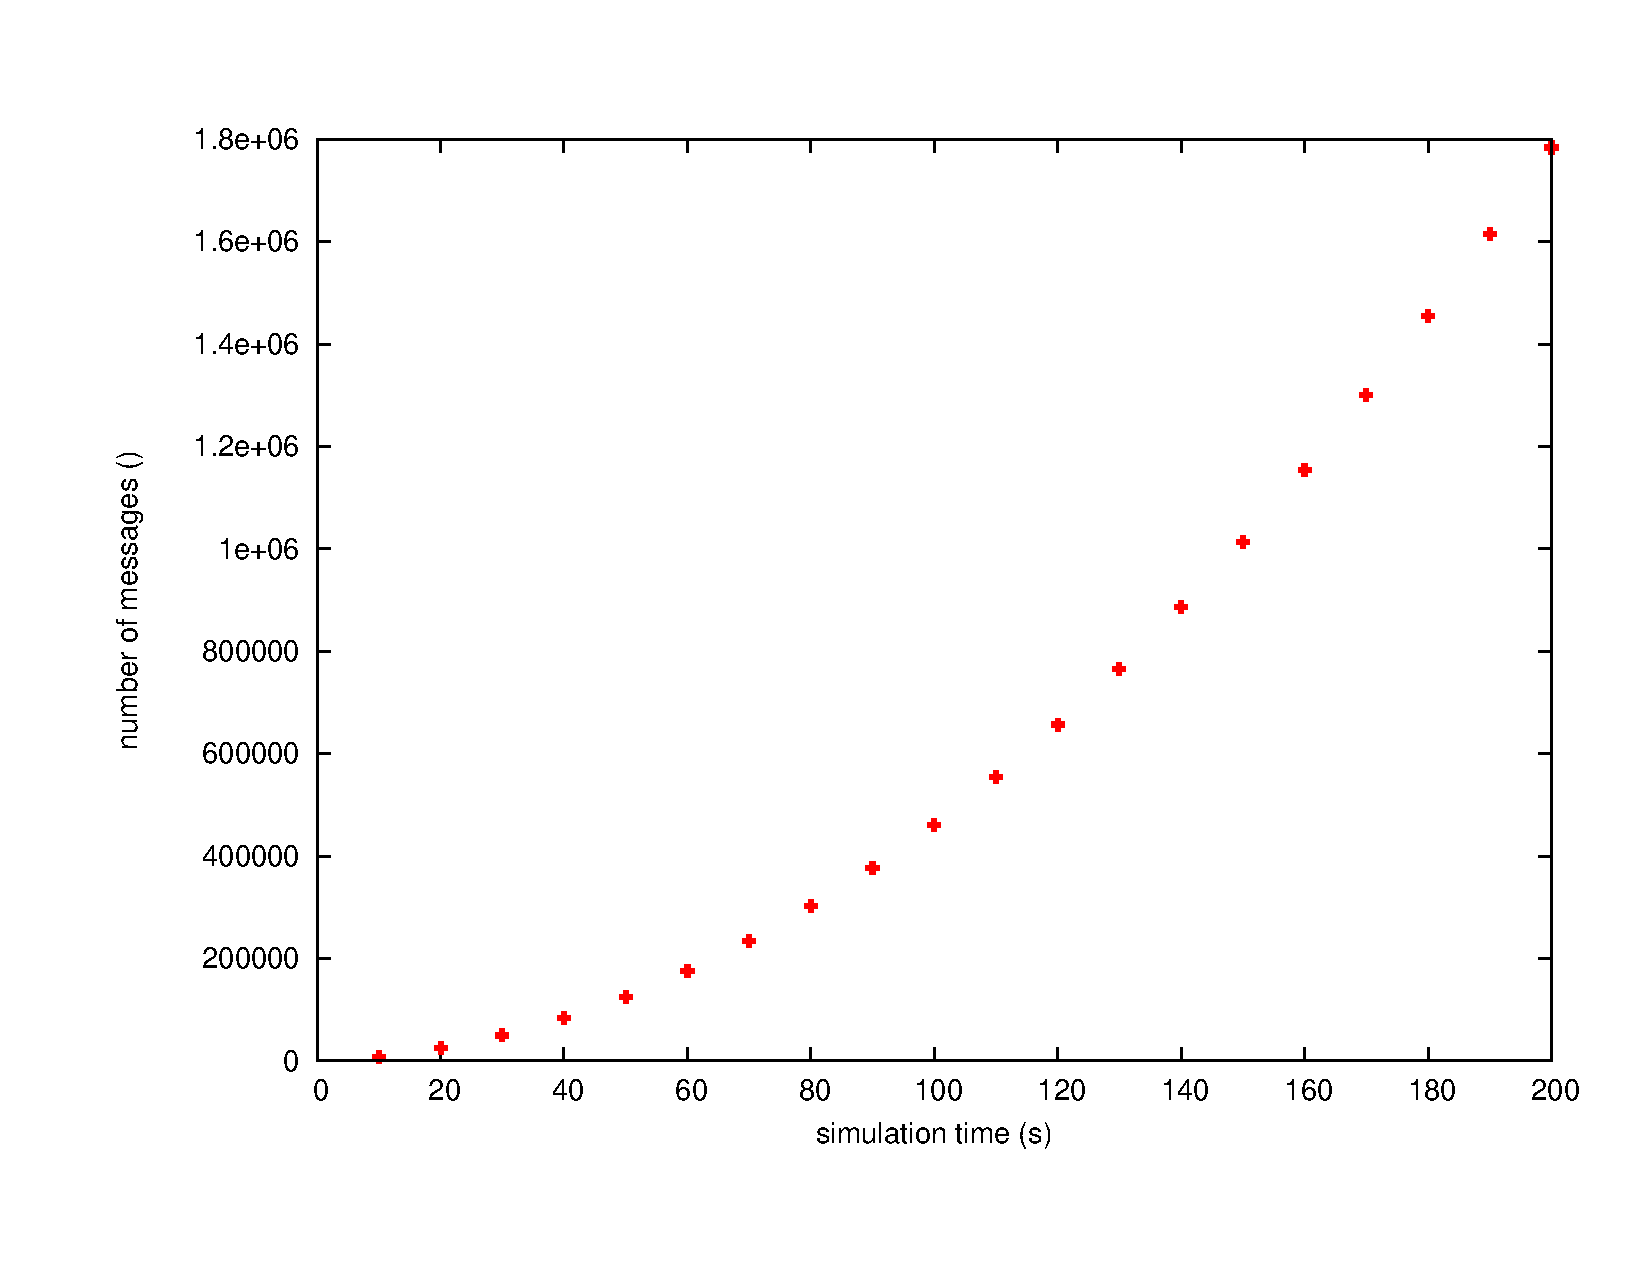
\includegraphics[scale=.3]{src/nbsimul-message}
      \label{timesim:message}
    }
    
    \subfigure[Moyenne de place]{
      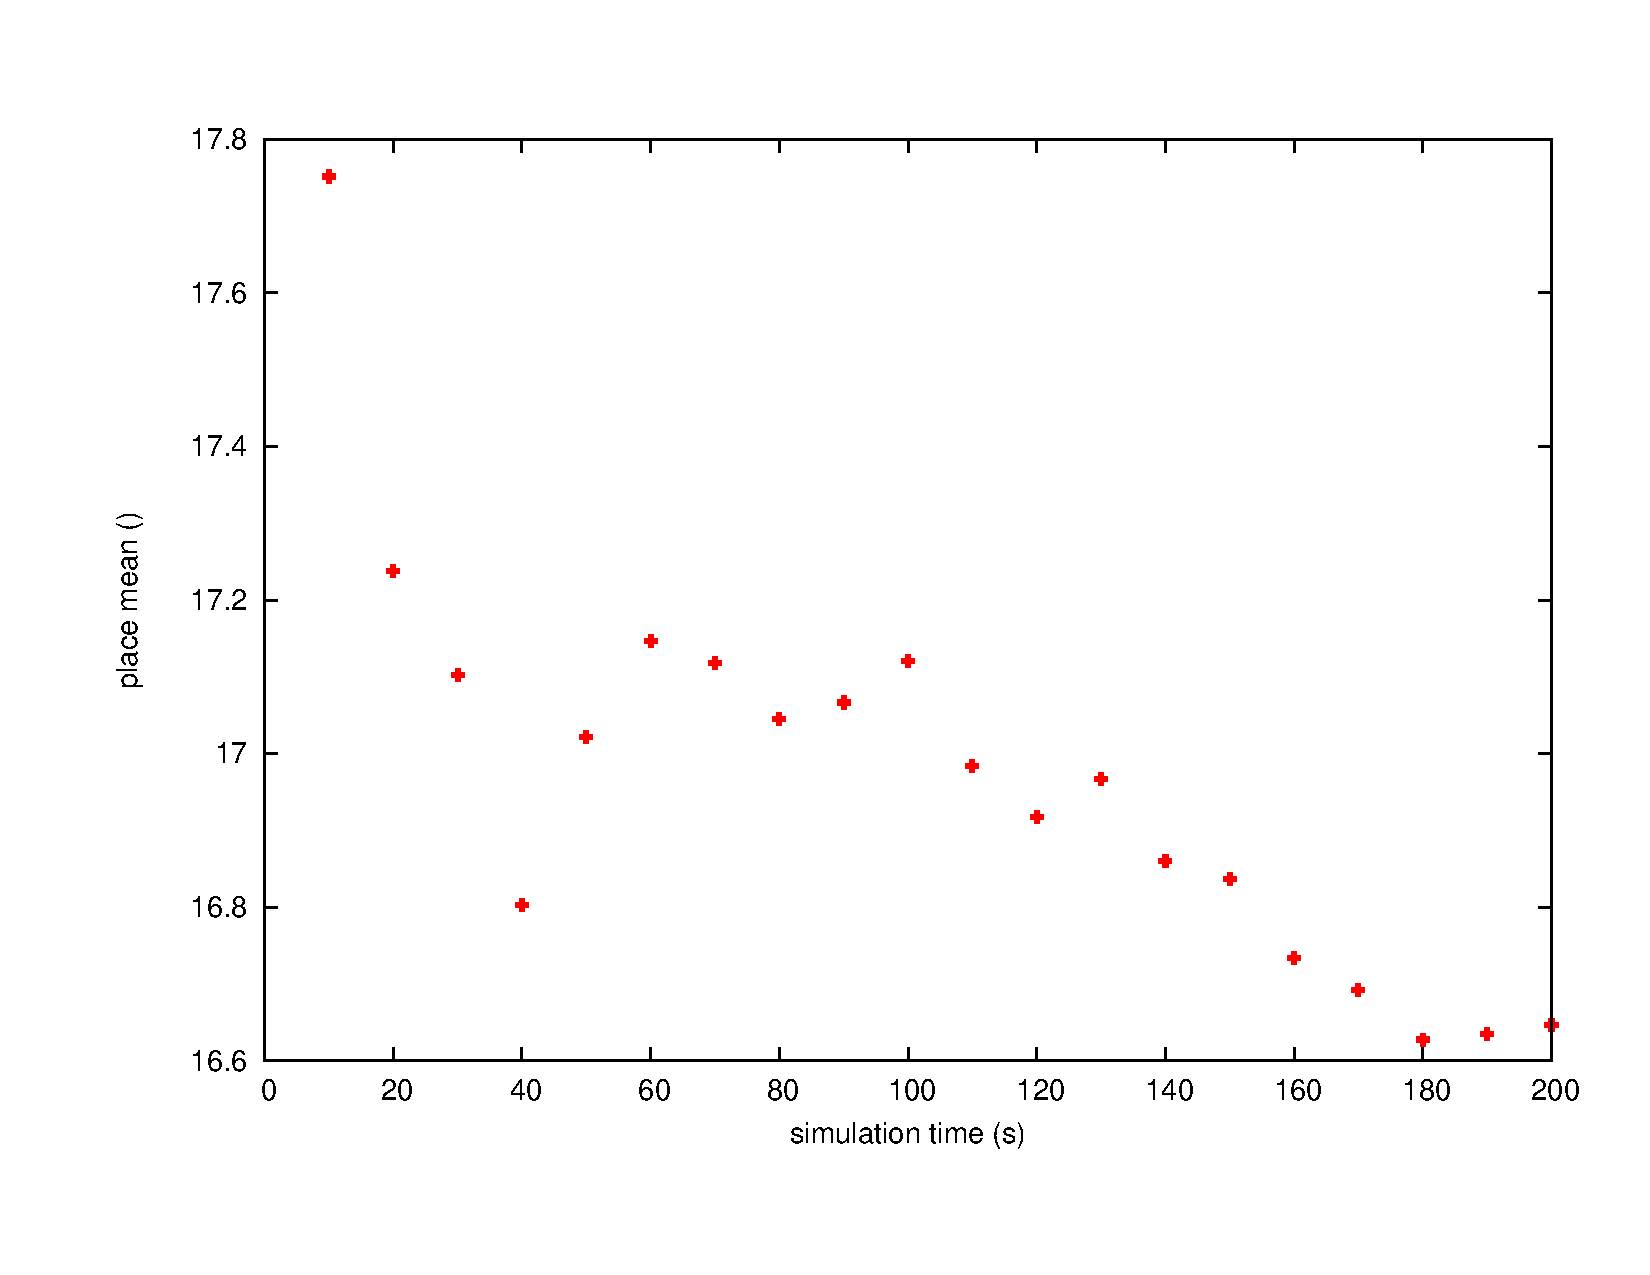
\includegraphics[scale=.3]{src/nbsimul-seekfound}
      \label{timesim:seekfound}
    }
    
    \subfigure[Ratio temps garé / temps total]{
      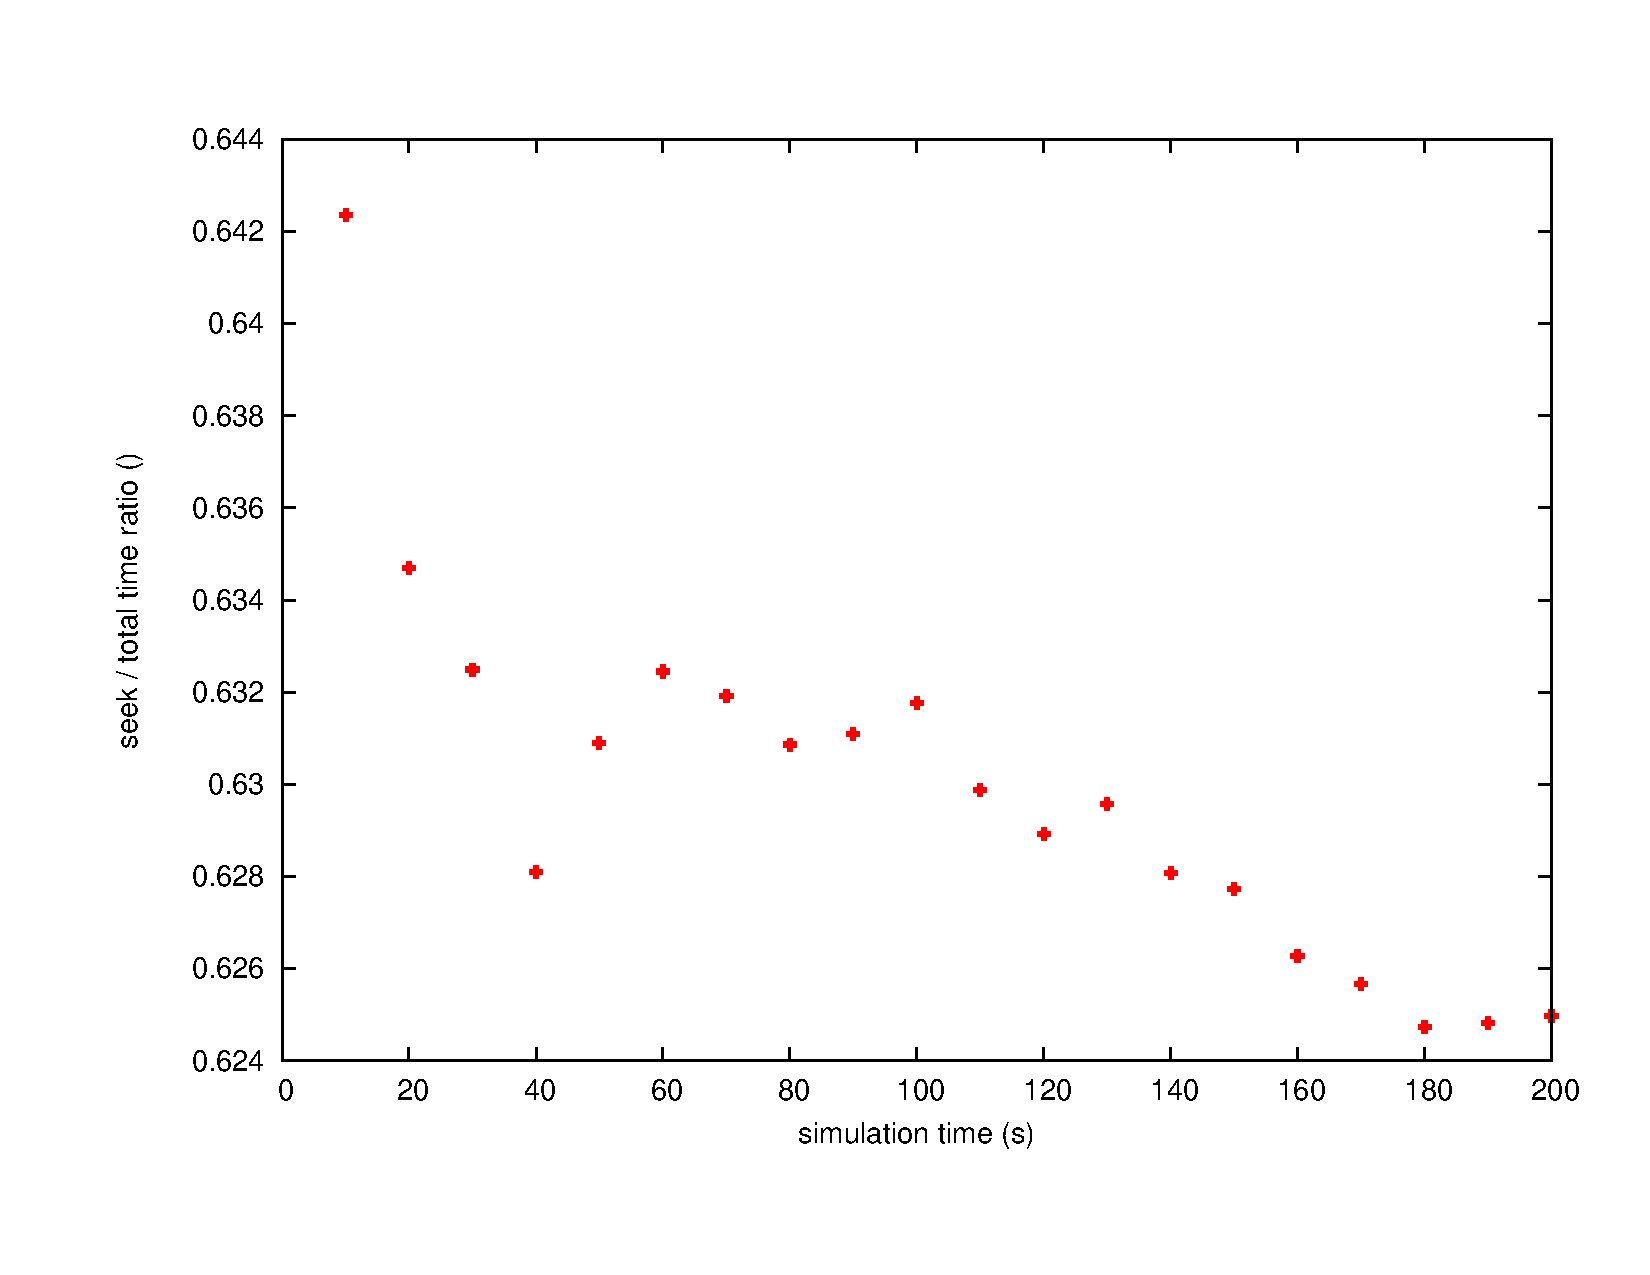
\includegraphics[scale=.3]{src/nbsimul-seeking}
      \label{timesim:seeking}
    }
  \end{center}

  \caption{Résultats obtenus en faisant varier la durée de la simulation (en s)}
  \label{timesim:all}
\end{figure}

\subsection{Comparaison avec un agent aléatoire}

La comparaison avec un agent aléatoire permet de voire l'amélioration apportée par notre solution.
Pour les paramètres standards donnés ci-dessus on a les valeurs suivantes sur une simulation de 200 secondes.

\begin{center}
  \begin{tabular}{c|c|c|c}
    & messages      & moyenne de place & $\frac{\mbox{temps recherche}}{\mbox{temps total}}$\\
    \hline
    Agent Aléatoire & 0        & 101.47                            & 0.90\\
    \hline
    Notre solution  & 234107   & 16.31                             & 0.62\\
  \end{tabular}
\end{center}

On observe que notre solution donne de bien meilleur résultats en terme de qualité du résultat mais est beaucoup plus coûteuse en terme de performances. La défaut principale de notre solution est que son efficacité varie beaucoup en fonction des paramètres propres aux agents. Par contre sa force est d'être assez invariables aux paramètres du système.

%%% Local Variables:
%%% mode: latex
%%% TeX-master: "../sma"
%%% compile-command: "cd ..; make"
%%% End:
